% Options for packages loaded elsewhere
\PassOptionsToPackage{unicode}{hyperref}
\PassOptionsToPackage{hyphens}{url}
\PassOptionsToPackage{dvipsnames,svgnames,x11names}{xcolor}
%
\documentclass[
  letterpaper,
  DIV=11,
  numbers=noendperiod]{scrartcl}

\usepackage{amsmath,amssymb}
\usepackage{iftex}
\ifPDFTeX
  \usepackage[T1]{fontenc}
  \usepackage[utf8]{inputenc}
  \usepackage{textcomp} % provide euro and other symbols
\else % if luatex or xetex
  \usepackage{unicode-math}
  \defaultfontfeatures{Scale=MatchLowercase}
  \defaultfontfeatures[\rmfamily]{Ligatures=TeX,Scale=1}
\fi
\usepackage{lmodern}
\ifPDFTeX\else  
    % xetex/luatex font selection
\fi
% Use upquote if available, for straight quotes in verbatim environments
\IfFileExists{upquote.sty}{\usepackage{upquote}}{}
\IfFileExists{microtype.sty}{% use microtype if available
  \usepackage[]{microtype}
  \UseMicrotypeSet[protrusion]{basicmath} % disable protrusion for tt fonts
}{}
\makeatletter
\@ifundefined{KOMAClassName}{% if non-KOMA class
  \IfFileExists{parskip.sty}{%
    \usepackage{parskip}
  }{% else
    \setlength{\parindent}{0pt}
    \setlength{\parskip}{6pt plus 2pt minus 1pt}}
}{% if KOMA class
  \KOMAoptions{parskip=half}}
\makeatother
\usepackage{xcolor}
\setlength{\emergencystretch}{3em} % prevent overfull lines
\setcounter{secnumdepth}{-\maxdimen} % remove section numbering
% Make \paragraph and \subparagraph free-standing
\makeatletter
\ifx\paragraph\undefined\else
  \let\oldparagraph\paragraph
  \renewcommand{\paragraph}{
    \@ifstar
      \xxxParagraphStar
      \xxxParagraphNoStar
  }
  \newcommand{\xxxParagraphStar}[1]{\oldparagraph*{#1}\mbox{}}
  \newcommand{\xxxParagraphNoStar}[1]{\oldparagraph{#1}\mbox{}}
\fi
\ifx\subparagraph\undefined\else
  \let\oldsubparagraph\subparagraph
  \renewcommand{\subparagraph}{
    \@ifstar
      \xxxSubParagraphStar
      \xxxSubParagraphNoStar
  }
  \newcommand{\xxxSubParagraphStar}[1]{\oldsubparagraph*{#1}\mbox{}}
  \newcommand{\xxxSubParagraphNoStar}[1]{\oldsubparagraph{#1}\mbox{}}
\fi
\makeatother


\providecommand{\tightlist}{%
  \setlength{\itemsep}{0pt}\setlength{\parskip}{0pt}}\usepackage{longtable,booktabs,array}
\usepackage{calc} % for calculating minipage widths
% Correct order of tables after \paragraph or \subparagraph
\usepackage{etoolbox}
\makeatletter
\patchcmd\longtable{\par}{\if@noskipsec\mbox{}\fi\par}{}{}
\makeatother
% Allow footnotes in longtable head/foot
\IfFileExists{footnotehyper.sty}{\usepackage{footnotehyper}}{\usepackage{footnote}}
\makesavenoteenv{longtable}
\usepackage{graphicx}
\makeatletter
\def\maxwidth{\ifdim\Gin@nat@width>\linewidth\linewidth\else\Gin@nat@width\fi}
\def\maxheight{\ifdim\Gin@nat@height>\textheight\textheight\else\Gin@nat@height\fi}
\makeatother
% Scale images if necessary, so that they will not overflow the page
% margins by default, and it is still possible to overwrite the defaults
% using explicit options in \includegraphics[width, height, ...]{}
\setkeys{Gin}{width=\maxwidth,height=\maxheight,keepaspectratio}
% Set default figure placement to htbp
\makeatletter
\def\fps@figure{htbp}
\makeatother
% definitions for citeproc citations
\NewDocumentCommand\citeproctext{}{}
\NewDocumentCommand\citeproc{mm}{%
  \begingroup\def\citeproctext{#2}\cite{#1}\endgroup}
\makeatletter
 % allow citations to break across lines
 \let\@cite@ofmt\@firstofone
 % avoid brackets around text for \cite:
 \def\@biblabel#1{}
 \def\@cite#1#2{{#1\if@tempswa , #2\fi}}
\makeatother
\newlength{\cslhangindent}
\setlength{\cslhangindent}{1.5em}
\newlength{\csllabelwidth}
\setlength{\csllabelwidth}{3em}
\newenvironment{CSLReferences}[2] % #1 hanging-indent, #2 entry-spacing
 {\begin{list}{}{%
  \setlength{\itemindent}{0pt}
  \setlength{\leftmargin}{0pt}
  \setlength{\parsep}{0pt}
  % turn on hanging indent if param 1 is 1
  \ifodd #1
   \setlength{\leftmargin}{\cslhangindent}
   \setlength{\itemindent}{-1\cslhangindent}
  \fi
  % set entry spacing
  \setlength{\itemsep}{#2\baselineskip}}}
 {\end{list}}
\usepackage{calc}
\newcommand{\CSLBlock}[1]{\hfill\break\parbox[t]{\linewidth}{\strut\ignorespaces#1\strut}}
\newcommand{\CSLLeftMargin}[1]{\parbox[t]{\csllabelwidth}{\strut#1\strut}}
\newcommand{\CSLRightInline}[1]{\parbox[t]{\linewidth - \csllabelwidth}{\strut#1\strut}}
\newcommand{\CSLIndent}[1]{\hspace{\cslhangindent}#1}

\usepackage{float}
\usepackage{tabularray}
\usepackage[normalem]{ulem}
\usepackage{graphicx}
\UseTblrLibrary{booktabs}
\UseTblrLibrary{siunitx}
\NewTableCommand{\tinytableDefineColor}[3]{\definecolor{#1}{#2}{#3}}
\newcommand{\tinytableTabularrayUnderline}[1]{\underline{#1}}
\newcommand{\tinytableTabularrayStrikeout}[1]{\sout{#1}}
\KOMAoption{captions}{tableheading}
\makeatletter
\@ifpackageloaded{tcolorbox}{}{\usepackage[skins,breakable]{tcolorbox}}
\@ifpackageloaded{fontawesome5}{}{\usepackage{fontawesome5}}
\definecolor{quarto-callout-color}{HTML}{909090}
\definecolor{quarto-callout-note-color}{HTML}{0758E5}
\definecolor{quarto-callout-important-color}{HTML}{CC1914}
\definecolor{quarto-callout-warning-color}{HTML}{EB9113}
\definecolor{quarto-callout-tip-color}{HTML}{00A047}
\definecolor{quarto-callout-caution-color}{HTML}{FC5300}
\definecolor{quarto-callout-color-frame}{HTML}{acacac}
\definecolor{quarto-callout-note-color-frame}{HTML}{4582ec}
\definecolor{quarto-callout-important-color-frame}{HTML}{d9534f}
\definecolor{quarto-callout-warning-color-frame}{HTML}{f0ad4e}
\definecolor{quarto-callout-tip-color-frame}{HTML}{02b875}
\definecolor{quarto-callout-caution-color-frame}{HTML}{fd7e14}
\makeatother
\makeatletter
\@ifpackageloaded{caption}{}{\usepackage{caption}}
\AtBeginDocument{%
\ifdefined\contentsname
  \renewcommand*\contentsname{Table of contents}
\else
  \newcommand\contentsname{Table of contents}
\fi
\ifdefined\listfigurename
  \renewcommand*\listfigurename{List of Figures}
\else
  \newcommand\listfigurename{List of Figures}
\fi
\ifdefined\listtablename
  \renewcommand*\listtablename{List of Tables}
\else
  \newcommand\listtablename{List of Tables}
\fi
\ifdefined\figurename
  \renewcommand*\figurename{Figure}
\else
  \newcommand\figurename{Figure}
\fi
\ifdefined\tablename
  \renewcommand*\tablename{Table}
\else
  \newcommand\tablename{Table}
\fi
}
\@ifpackageloaded{float}{}{\usepackage{float}}
\floatstyle{ruled}
\@ifundefined{c@chapter}{\newfloat{codelisting}{h}{lop}}{\newfloat{codelisting}{h}{lop}[chapter]}
\floatname{codelisting}{Listing}
\newcommand*\listoflistings{\listof{codelisting}{List of Listings}}
\makeatother
\makeatletter
\makeatother
\makeatletter
\@ifpackageloaded{caption}{}{\usepackage{caption}}
\@ifpackageloaded{subcaption}{}{\usepackage{subcaption}}
\makeatother

\ifLuaTeX
  \usepackage{selnolig}  % disable illegal ligatures
\fi
\usepackage{bookmark}

\IfFileExists{xurl.sty}{\usepackage{xurl}}{} % add URL line breaks if available
\urlstyle{same} % disable monospaced font for URLs
\hypersetup{
  pdftitle={Services and the Third Unbundling in Indonesia},
  pdfauthor={Krisna Gupta; Dhany S. Ratana},
  colorlinks=true,
  linkcolor={blue},
  filecolor={Maroon},
  citecolor={Blue},
  urlcolor={Blue},
  pdfcreator={LaTeX via pandoc}}


\title{Services and the Third Unbundling in Indonesia}
\author{Krisna Gupta \and Dhany S. Ratana}
\date{October 27, 2024}

\begin{document}
\maketitle


\begin{tcolorbox}[enhanced jigsaw, colbacktitle=quarto-callout-warning-color!10!white, toprule=.15mm, coltitle=black, colback=white, opacitybacktitle=0.6, opacityback=0, title=\textcolor{quarto-callout-warning-color}{\faExclamationTriangle}\hspace{0.5em}{Warning}, bottomtitle=1mm, toptitle=1mm, colframe=quarto-callout-warning-color-frame, titlerule=0mm, rightrule=.15mm, arc=.35mm, bottomrule=.15mm, breakable, leftrule=.75mm, left=2mm]

This document is a work in progress. Please do not cite. Comments are
welcomed. For replication see
\href{https://github.com/imedkrisna/ERIA_services}{here}

\end{tcolorbox}

\subsection{Introduction}\label{introduction}

Trade in services is growing in importance all over the world, Indonesia
included. Figure~\ref{fig-1} shows Indonesia's export and import in
services taken from Indonesian Statistic Bureau compiled by the Central
Bank (Bank Indonesia, n.d.). Indonesia's services trade is growing
steadily from 2000, only to be interrupted by the COVID-19 pandemic.
Export service is dominated by tourism, while import services is
dominated by logistics. While the trend is increasing, it is evident
that Indonesia's import of services has always been dominating exports.

\begin{figure}

\centering{

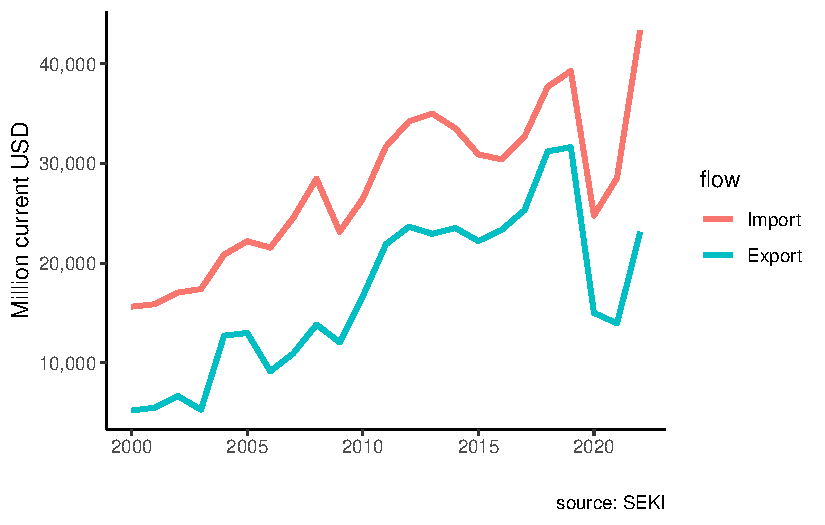
\includegraphics{services_document_files/figure-pdf/fig-1-1.pdf}

}

\caption{\label{fig-1}Indonesian trade in services}

\end{figure}%

Indonesian government often concerned with deficit trade, but trade in
services has often neglected in the discussion. Indeed, trade balance in
goods are often far outweight the deficit in its services counterpart,
as made apparent by Figure~\ref{fig-2}. However, while Indonesia's trade
balance fluctuates along with commodity prices and global demand in
general, services trade deficit is consistent. Additionally, Indonesia's
reliance on services import went up right after COVID-19 and seems to
stabilize in a higher than pre-pandemic level. With the increasing role
of services in the global trade, the deficit looks to be even more
important in Indonesia's current account in the future.

\begin{figure}

\centering{

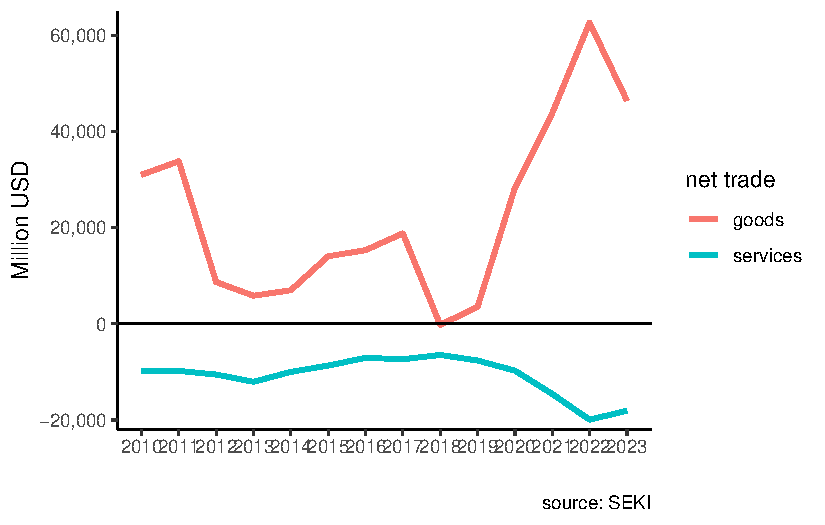
\includegraphics{services_document_files/figure-pdf/fig-2-1.pdf}

}

\caption{\label{fig-2}Net trade in goods and services of Indonesia, 200}

\end{figure}%

The importance of trade in services goes beyond current account. With
the ever decreasing cost of trade, separating a value up to tasks level
(i.e., the third unbundling) is on the horizon (Baldwin 2011; Kimura
2018). Feedback mechanism from the third unbundling may benefits
domestic manufacturing (Kimura 2018). Therefore, services trade may be
important in the next stage of globalization.

Even by itself, trade in services seems to be the new future for
developing countries (Baldwin 2011; Aiginger and Rodrik 2020). While
trade in goods has been stagnating since 2011, trade in services
continues to grow (see Figure~\ref{fig-trade}). The scale is indeed
small, but the growth is consistent. With the expected trade cost for
services and technologies to facilitate services trade grow, trade in
services is expected to drive the development of countries missing the
first two unbundlings.

\begin{figure}

\begin{minipage}{0.50\linewidth}

\centering{

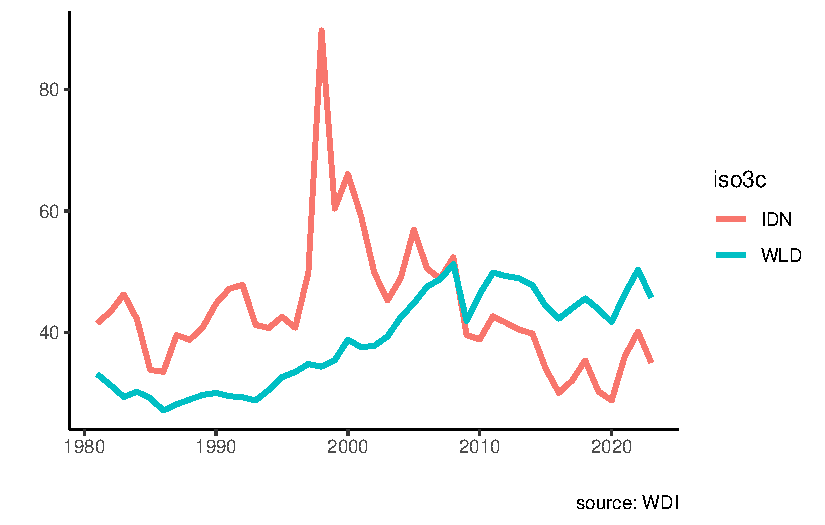
\includegraphics{services_document_files/figure-pdf/fig-trade-1.pdf}

}

\subcaption{\label{fig-trade-1}World trade (\% of GDP)}

\end{minipage}%
%
\begin{minipage}{0.50\linewidth}

\centering{

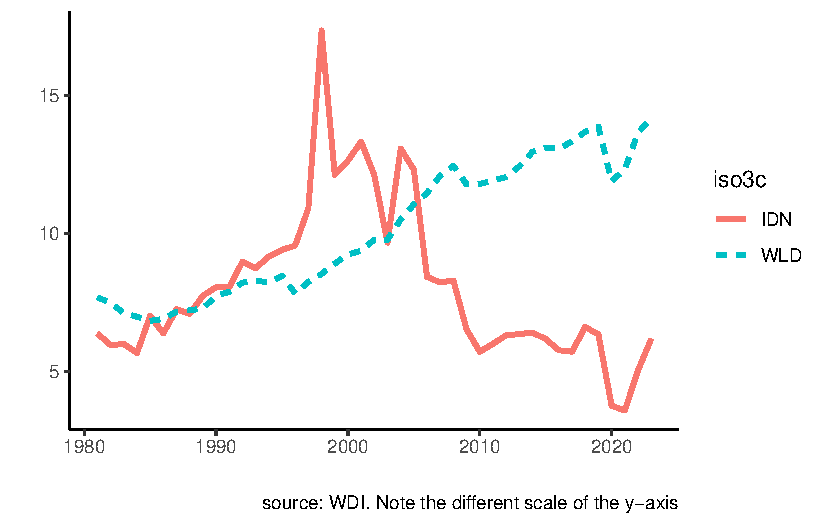
\includegraphics{services_document_files/figure-pdf/fig-trade-2.pdf}

}

\subcaption{\label{fig-trade-2}Indonesian trade (\% of GDP)}

\end{minipage}%

\caption{\label{fig-trade}Goods and services trade in Indonesia and the
World}

\end{figure}%

Indonesia, some argue, has missed the opportunity of the globalization
of production network Hill and Pane (2018). The next form of
globalization, thus, should be optimized by Indonesia. As seen in the
Figure~\ref{fig-trade}, however, Indonesia seems to going to miss the
services train as well. Trade in services in Indonesia is
underdeveloped, and barriers to entry for services trade remains high
(Magiera 2011; Patunru 2023).

This chapter have at least two objectives. First, we explores the
general trade in services in Indonesia. We use BaTIS data (WTO/OECD
2022; Liberatore and Wettstein 2021) to show Indonesia's most important
services trade and country partners for both export and import. We also
use ICIO (\textbf{ICIO?}) to show how important services are to
manufacturing, both domestic and foreign.

Secondly, we look at the development of Indonesia's regulations related
to trade in services. We extend Magiera (2011) to examine Indonesia's
development in regulatory practices around trade in services. We find
the importance of foreign direct investment in opening trade in
services, and show that relaxation of services stringency index seemed
to stem from relaxation of foreign ownership restrictions in Indonesia's
service sector. Additionally, relaxing trade in services in Indonesia is
more complicated amid involvement of number of ministries magnitudes
higher than ones involved in tariff reduction.

We arrange this chapter in the following. Section 2 discusses the
development in research concerning services trade and its development in
Indonesia, section 3 discusses about data and methods, section 4
explores Indonesian services trade as well as some third unbundling
results, and section 5 concludes.

\subsection{Review on services trade}\label{review-on-services-trade}

The concept of trade has been evolving from the the way goods (and later
services) value chain can be broken. Baldwin (2016) coined the term
``unbundling'' to express the variety of trade can be done by how much
part of the supply chain of production can be traded across border.
Lower costs in various trade barriers (trade costs, communication costs,
and face-to-face costs) leads to more possible breakdowns of a value
chain, promotes better division of tasks.

Kimura (2018) use this concept to argue three possible development paths
for ASEAN member states to take. A country can move slowly, step-by-step
by lowering trade cost traditionally from agriculture to machinaries to
digital economy. One can also take a leap-frogging path, directly
joining Global Value Chain by starting in the downstream, or even go
directly to services trade, which is available through unbundling tasks
in the service sectors. Lastly, A country can do a feedback mechanism,
where advanced technology changes how old industries work. Looking at
the last two approaches, services trade can be utilize either by
learning from manufacturing to services export, or using services to
create a better manufacturing.

Now with trade cost is even lower, unbundling the service sector become
feasible. Some firms allowing some firms to leap ahead (Kimura 2018).
Trade in services can be either source from abroad, or exported to
foreign firms. Service sectors will accelerate both the second
unbundling or third unbundling, allowing firms that utilize it to leap
ahead of the competition.

Service sector can provide an important advantage for many firms,
especially manufacturing ones. It can brigde information gap on the
market, business customs and regulations in other countries, especially
for new firms entering export market (Lodefalk 2014). As has been shown
by (Melitz 2003), a non-trivial trade cost limits firm who can enter the
export market. A reduction in trade cost in services would help lower
the productivity threshold for firms, enabling more to enter the export
market. This entrance would then induce learning-by-doing for these low
productivity firms.

Lodefalk (2014) study Sweeden's manufacturing firm in 2001-2007. They
conclude that firms with higher services embeded in its final products
increases its intensity of export. In the Indonesian context, Hing and
Thangavelu (2023) find that 10 per cent increase in service intensity of
a firm increase its productivity by 7 to 8 per cent. The two papers use
firms level data with information on what services each firm purchase.
Information on whether the service is imported, however, is lacking.

Lower services cost can reduce firms' cost of service outsourcing. In
the Indonesian context, Syahputri and Gupta (2024) uses gravity in
service trade approach (Kimura 2018) to see whether IJEPA helps with
improving Indonesia's trade in services. Utilizing services data from
BaTIS, Syahputri and Gupta (2024) find that IJEPA, one of the first
comprehensive economic agreement in Indonesia, does not increase service
trade between the two countries.

Indonesia does not seem to use services a lot. Services account for only
around 2\% of Indonesian manufacturing firms' output (Hing and
Thangavelu 2023), Indonesia's trade in services is also falls short.
Services trade requires easing in four different modes. Therefore,
regulations typically rarely discussed in a trade agreement such as
investment impediment, movement of natural persons and technical barrier
all makes service trade much harder (Syahputri and Gupta 2024; Magiera
2011).

With \emph{hilirisasi} or downstreaming policy, tendency to reduce
import is more apparent. This policy's objective was to increase the
added value of the manufacturing sector by reducing foreign content in
the domestic value chain. Local Content Requirements (LCR) put emphasize
on domestic value added which means making production in the same
area/country, running counter to joining internationally oriented global
value chains/GVCs (Athukorala and Patunru 2023). GVCs involve dividing
up production process across borders, equivalent of the second
unbundling. Thus, hilirisasi and LCR policies ended up bundling up
production processes that could be divvied up among countries. This
meant undoing the second unbundling, let alone encouraging the third
unbundling.

\subsection{Data and Method}\label{data-and-method}

There are two main dataset used in this chapter. Namely, Balanced Trade
in Services (BaTIS) and the OECD Inter-Country Input-Output (ICIO)
dataset.

The BaTIS database was first launched in 2017 by World Trade
organization (WTO) and Organization of Economic Cooperation and
Development (OECD) in tandem (Liberatore and Wettstein 2021). Unlike
trade in goods, trade in services are harder to track than trade in
goods amid gap in data collection by various countries. BaTIS collect
both ways from pairs of trading partners, reconcile difference between
reporting countries' trade. BaTIS is also used to build Trade in Value
Added (TiVA) database and the ICIO database. BaTIS follows EBOPS 2010
sector classification (Liberatore et al. 2021) which can be observed in
Table~\ref{tbl-1}.

\begin{longtable}[]{@{}ll@{}}
\caption{Services classification in BaTIS}\label{tbl-1}\tabularnewline
\toprule\noalign{}
Code & Category description \\
\midrule\noalign{}
\endfirsthead
\toprule\noalign{}
Code & Category description \\
\midrule\noalign{}
\endhead
\bottomrule\noalign{}
\endlastfoot
SA & Manufacturing services on physical inputs owned by others \\
SB & Maintenance and repair services n.i.e. \\
SC & Transport \\
SD & Travel \\
SE & Construction \\
SF & Insurance and pension services \\
SG & Financial services \\
SH & Charges for the use of intellectual property n.i.e. \\
SI & Telecommunications, computer, and information services \\
SJ & Other business services \\
SK & Personal, cultural and recreational services \\
SL & Government goods and services n.i.e. \\
\end{longtable}

Trade services statistics are challenging in nature (Liberatore and
Wettstein 2021). Only around 65\% of total number of trade in services
are recorded bilaterally. Unlike trade in goods, exports are recoreded
better than imports, mainly due to advance countries being the majority
of service exporters. Only 59\% of trade value in BaTIS are fully
reported, which are the reported 65\% pair. The remaining 41\% are
estimated using share interpolations and gravity estimations. Since
BaTIS is used for other databases including TiVA and ICIO, we should
expect similar problems in these two databases.

Additionally, we also use the Indonesian trade in services statistics
compiled by the Indonesian central bank called \emph{Statistik Ekonomi
dan Keuangan Indonesia} (SEKI) (Bank Indonesia, n.d.). It records
Indonesia's trade in services in the same manner as BaTIS, but with less
detail on the trading partners. Moreover, SEKI is also used to observe
Indonesia's manufacturing GDP and goods exports and imports to estimate
the third unbundling effect.

The OECD Inter-Country Input-Output (ICIO) decribes the sale and
purchase relationships between sectors, consumers and the government
within and across borders. ICIO estimates trades amonng 76 countries and
45 unique industries based on ISIC Revision 4(OECD, 2023). The database
shows how much sectoral value added, both foreign and domestic, that is
used by a certain industry.

In this study, we focus the manufacturing sector, specifically ISIC
10-27 in the ISIC rev. 4 classification. The ICIO aggregates these
sectors into 16 sectors. We then aggregates all services that sell to
these sectors into two categories, namely domestic services and foreign
services.

On the third unbundling discussion, a good quality of firm-level data
with information of its services sourced. Unfortunately, this
information is not widely distributed in the Indonesian context. The
second-best approach is to use international input-output table, which
in this case ICIO is used.

Assume a manufacturing output and value added as a function of its
factor or production. The nest of factor of production produces fully
complementarily with its goods and services inputs. Let services inputs
be complementarily used with goods inputs, but within the value produced
by services, there is a degree of substitutability between foreign and
domestic input as such:

\begin{equation}\phantomsection\label{eq-1}{
Y_{it}=f(AS^D_{it},AS^F_{it})
}\end{equation}

for all \(i=\) manufacturing sectors and \(t=year\). A is the nest
multiplier, \(S^D_i\) and \(S^F_i\) are total services purchased by
industry \(i\), domestically and imported respectively.

Assuming a cobb-douglass relationship, then we can log-linearize
Equation~\ref{eq-1} to a simple linear system as such:

\begin{equation}\phantomsection\label{eq-2}{
y_{it}=a+\beta_d s^D_{it}+\beta_f s^F_{it}+\varepsilon_{it}
}\end{equation}

with a lower case represents the natural log of its uppercase
counterpart.

To construct the dataset for the regression, we aggregate non-factor
inputs from each manufacuring sectors, separated by whether it is from
Indonesia or from other countries. All inputs from foreign countries are
aggregated into foreign.

For comparison purpose, we also do the same for 4 countries in the
region, namely Singapore, Malaysia, Thailand and Vietnam. Data from
these 5 countries are then concatenated to add one more dimension,
countries. Summary statistics on the data is shown in
Table~\ref{tbl-icio}.

\begin{table}

\caption{\label{tbl-icio}Summary Statistics from ICIO, million USD,
2002-2021.}

\centering{

\centering
\begin{tblr}[         %% tabularray outer open
]                     %% tabularray outer close
{                     %% tabularray inner open
colspec={Q[]Q[]Q[]Q[]Q[]Q[]Q[]},
cell{1}{2}={c=3,}{halign=c,},
cell{1}{5}={c=3,}{halign=c,},
column{1}={halign=l,},
column{2}={halign=r,},
column{3}={halign=r,},
column{4}={halign=r,},
column{5}={halign=r,},
column{6}={halign=r,},
column{7}={halign=r,},
row{1}={halign=c,},
}                     %% tabularray inner close
\toprule
& all &  &  & IDN &  &  \\ \cmidrule[lr]{2-4}\cmidrule[lr]{5-7}
& Mean & SD & Histogram & Mean & SD & Histogram \\ \midrule %% TinyTableHeader
value added         & \num{4181.70}  & \num{6845.40}  & ▇▁        & \num{8150.56}  & \num{12191.95} & ▇▁         \\
output              & \num{15930.67} & \num{21741.55} & ▇▁        & \num{21529.33} & \num{29317.48} & ▇▁▁        \\
domestic services   & \num{2804.36}  & \num{3889.86}  & ▇▂▁       & \num{3735.21}  & \num{4176.07}  & ▇▅▁        \\
foreign services    & \num{845.74}   & \num{1730.29}  & ▇         & \num{420.05}   & \num{339.95}   & ▇▆▄▃▂▁     \\
domestic goods      & \num{5213.09}  & \num{9008.54}  & ▇▁        & \num{7123.05}  & \num{12296.21} & ▇▁         \\
foreign goods       & \num{7057.46}  & \num{9172.47}  & ▇▁▁       & \num{10240.63} & \num{12983.59} & ▇▁▁        \\
for. services share & \num{5.76}     & \num{3.70}     & ▃▇▃▁      & \num{2.45}     & \num{1.34}     & ▇▆▆▇▄▃▂▂▁  \\
dom. services share & \num{18.02}    & \num{6.73}     & ▂▇▇▇▅▃▁▁  & \num{18.55}    & \num{5.41}     & ▂▆▇▇▅▄▅▃▁  \\
for. goods share    & \num{47.62}    & \num{11.39}    & ▁▂▂▅▇▆▄▂▁ & \num{50.30}    & \num{11.98}    & ▁▁▃▇▅▇▅▁▂▁ \\
dom. goods share    & \num{28.37}    & \num{11.11}    & ▃▄▇▇▄▂    & \num{28.60}    & \num{8.57}     & ▁▂▂▃▅▇▅▄▂▁ \\
\bottomrule
\end{tblr}

}

\end{table}%

Table~\ref{tbl-icio} shows Average and standard deviation as well as
distribution of value added, output, domestic and foreign goods and
services value and share. Unsurprisingly Indonesian manufacturing output
and value added is higher than average of 5 countries, amid how large
Indonesia is compared to its neighbor. Interestingly, Indonesian
manufacturing value added from foreign goods and share is larger than
the average, despite Indonesia's protectionist tendency (Patunru 2023).
Services, on the other hand, is different, as Indonesian services import
lags compared to other countries.

Lastly, we run 6 fixed effect panel regressions. The first panel
consists of two indices, country and sector, which both dummies are used
as a fixed effect. The other 5 panels are fixed effect regressions by
country, where only sectoral fixed effect is used. This way, we can
discuss difference in coefficient between selected countries in the
region. We use output and value added as our \(y_i\), so we will have 12
fixed effect panel regressions in total.

The main variable of interest is \(\beta_f\). The third unbundling
suggests that since firms can now unbundle tasks up to service level,
firms who can unbundle its services tasks will theoretically perform
better, shown in its value added and output. Likewise, industries with
easier services unbundling will benefited more from services trade since
there will be more firms able to exploit the third unbundling in these
industries. Therefore, we expect to see a \(\beta_f>0\).

Given the limitation of ICIO and its underlying sources (i.e., BaTIS),
macro level analysis is added to complement the analysis. We use SEKI,
Indonesian database compiled by Bank Indonesia, the central bank, to get
services trade, manufactures trade, and manufacturing output. We perform
ARDL analysis (Pesaran and Smith 1995) to see whether services trade
cointegrates with manufacturing output and export.

We run four specifications:

\begin{equation}\phantomsection\label{eq-3}{
\begin{align}
exM_t&=\alpha_0+\alpha_1 exM_{t-1}+\alpha_2 imM_t+\alpha_3 imSev_t+\nu_i \\
exM_t&=\gamma_0+\gamma_1 exM_{t-1}+\gamma_2 imM_t+\gamma_3 imSev_t+ \gamma_4 imM_{t-1}+\gamma_5 imSev_{t-1}+\upsilon_i \\
pdb_t&=\delta_0+\delta_1 exM_{t-1}+\delta_2 imM_t+\delta_3 imSev_t+\omega_i \\
pdb_t&=\theta_0+\theta_1 exM_{t-1}+\theta_2 imM_t+\theta_3 imSev_t+ \theta_4 imM_{t-1}+\theta_5 imSev_{t-1}+\eta_i
\end{align}
}\end{equation}

where \(exM\) is log manufacturing exports, \(pdb\) is log manufacturing
GDP, \(imM\) is log manufacturing imports and \(imSev\) is log services
imports, all for Indonesian level in time \(t\), where \(t\) is from
2005 to 2023. The data availability is restricted by the services import
which starts from 2005 in the SEKI data. Specifications that we run are
\texttt{ARDL(1,0,0)}, the least restrictive, and \texttt{ARDL(1,1,1)}
which is considered from AIC, BIC and RMSE (Pesaran and Smith 1995;
Natsiopoulos and Tzeremes 2022).

\subsection{Discussions}\label{discussions}

\subsubsection{Indonesian trade in
services}\label{indonesian-trade-in-services}

Figure~\ref{fig-S} shows total trade in services in 2021 in million
current USD taken from BaTIS. Categories are based on the
Table~\ref{tbl-1}. Figure~\ref{fig-CX} and Figure~\ref{fig-CM} shows
Indonesia's top 6 exporter and importer of services in 2021. Singapore
is the most important partner in trade in services for Indonesia. China,
on the other hand, is the main buyer of Indonesia's services export.
Looking at Figure~\ref{fig-SX} and Figure~\ref{fig-SM}, It is evident
that Indonesia's imports dominates exports in all categories bar travel
(SD). Additionally, the highest traded services in Indonesia are
transport (SC) and business services (SJ), aligned with global trade
statistics (Liberatore et al. 2021).

\begin{figure}

\begin{minipage}{0.50\linewidth}

\centering{

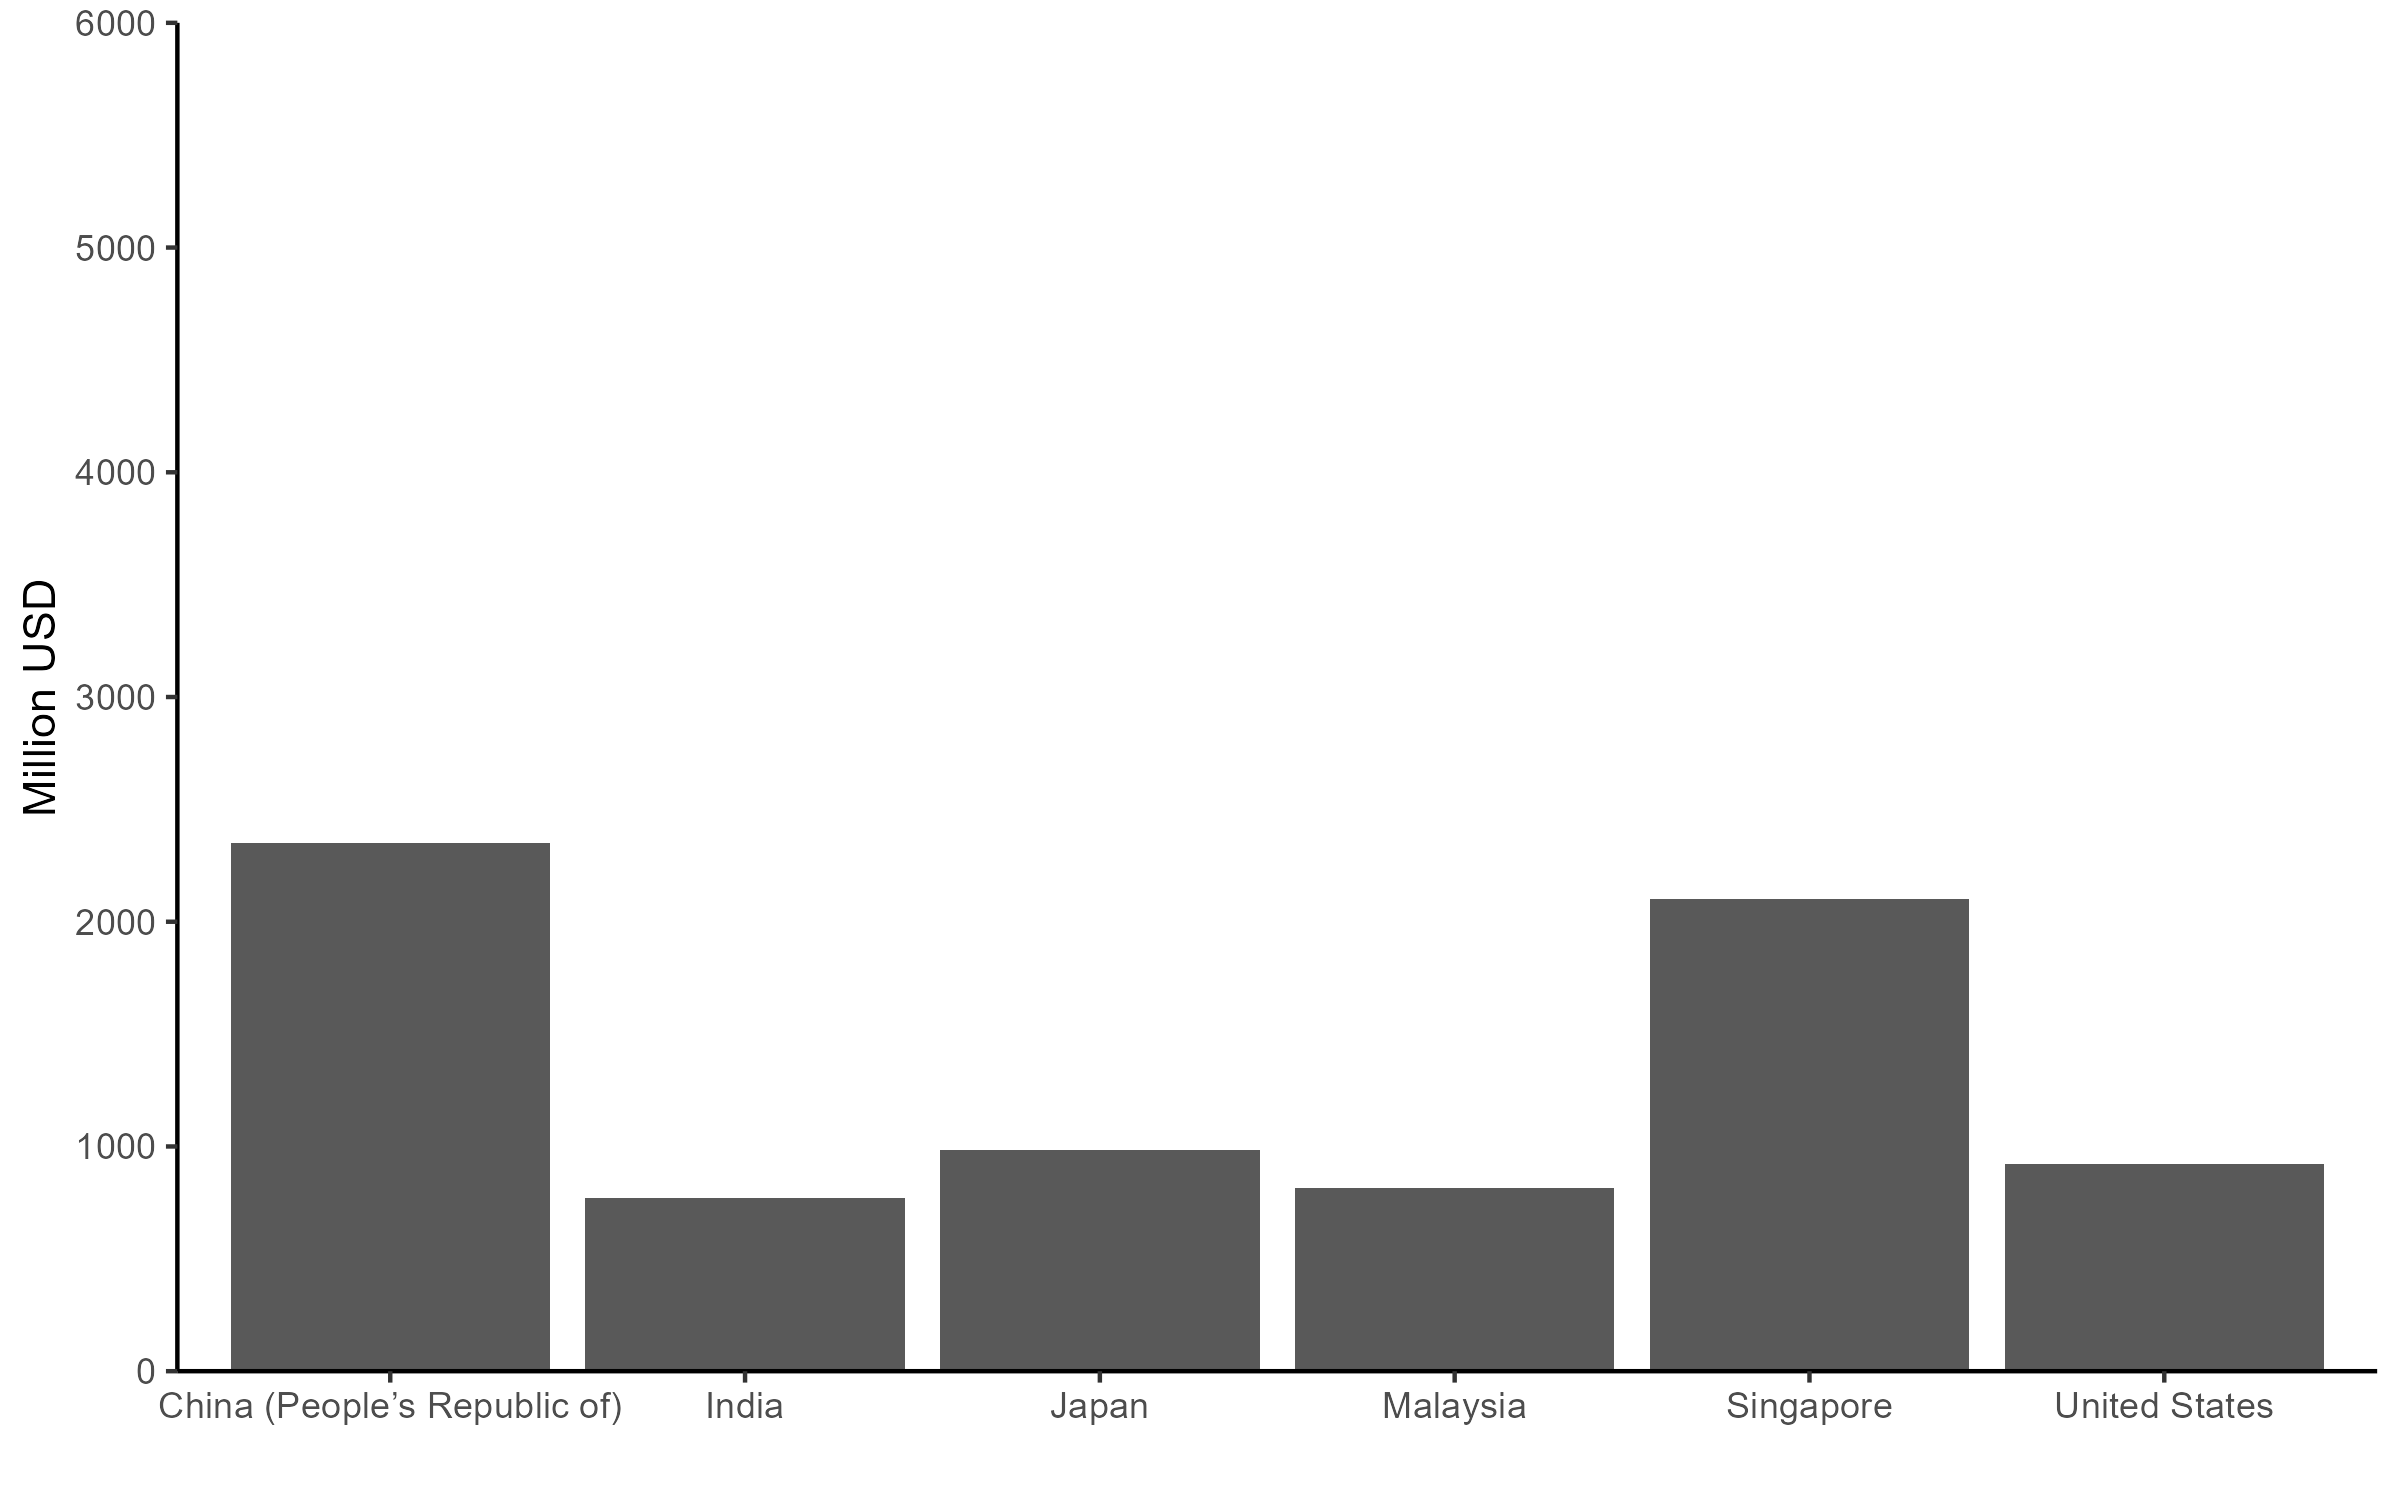
\includegraphics{plot/allcx.png}

}

\subcaption{\label{fig-CX}Indonesia's exports by partner, 2021}

\end{minipage}%
%
\begin{minipage}{0.50\linewidth}

\centering{

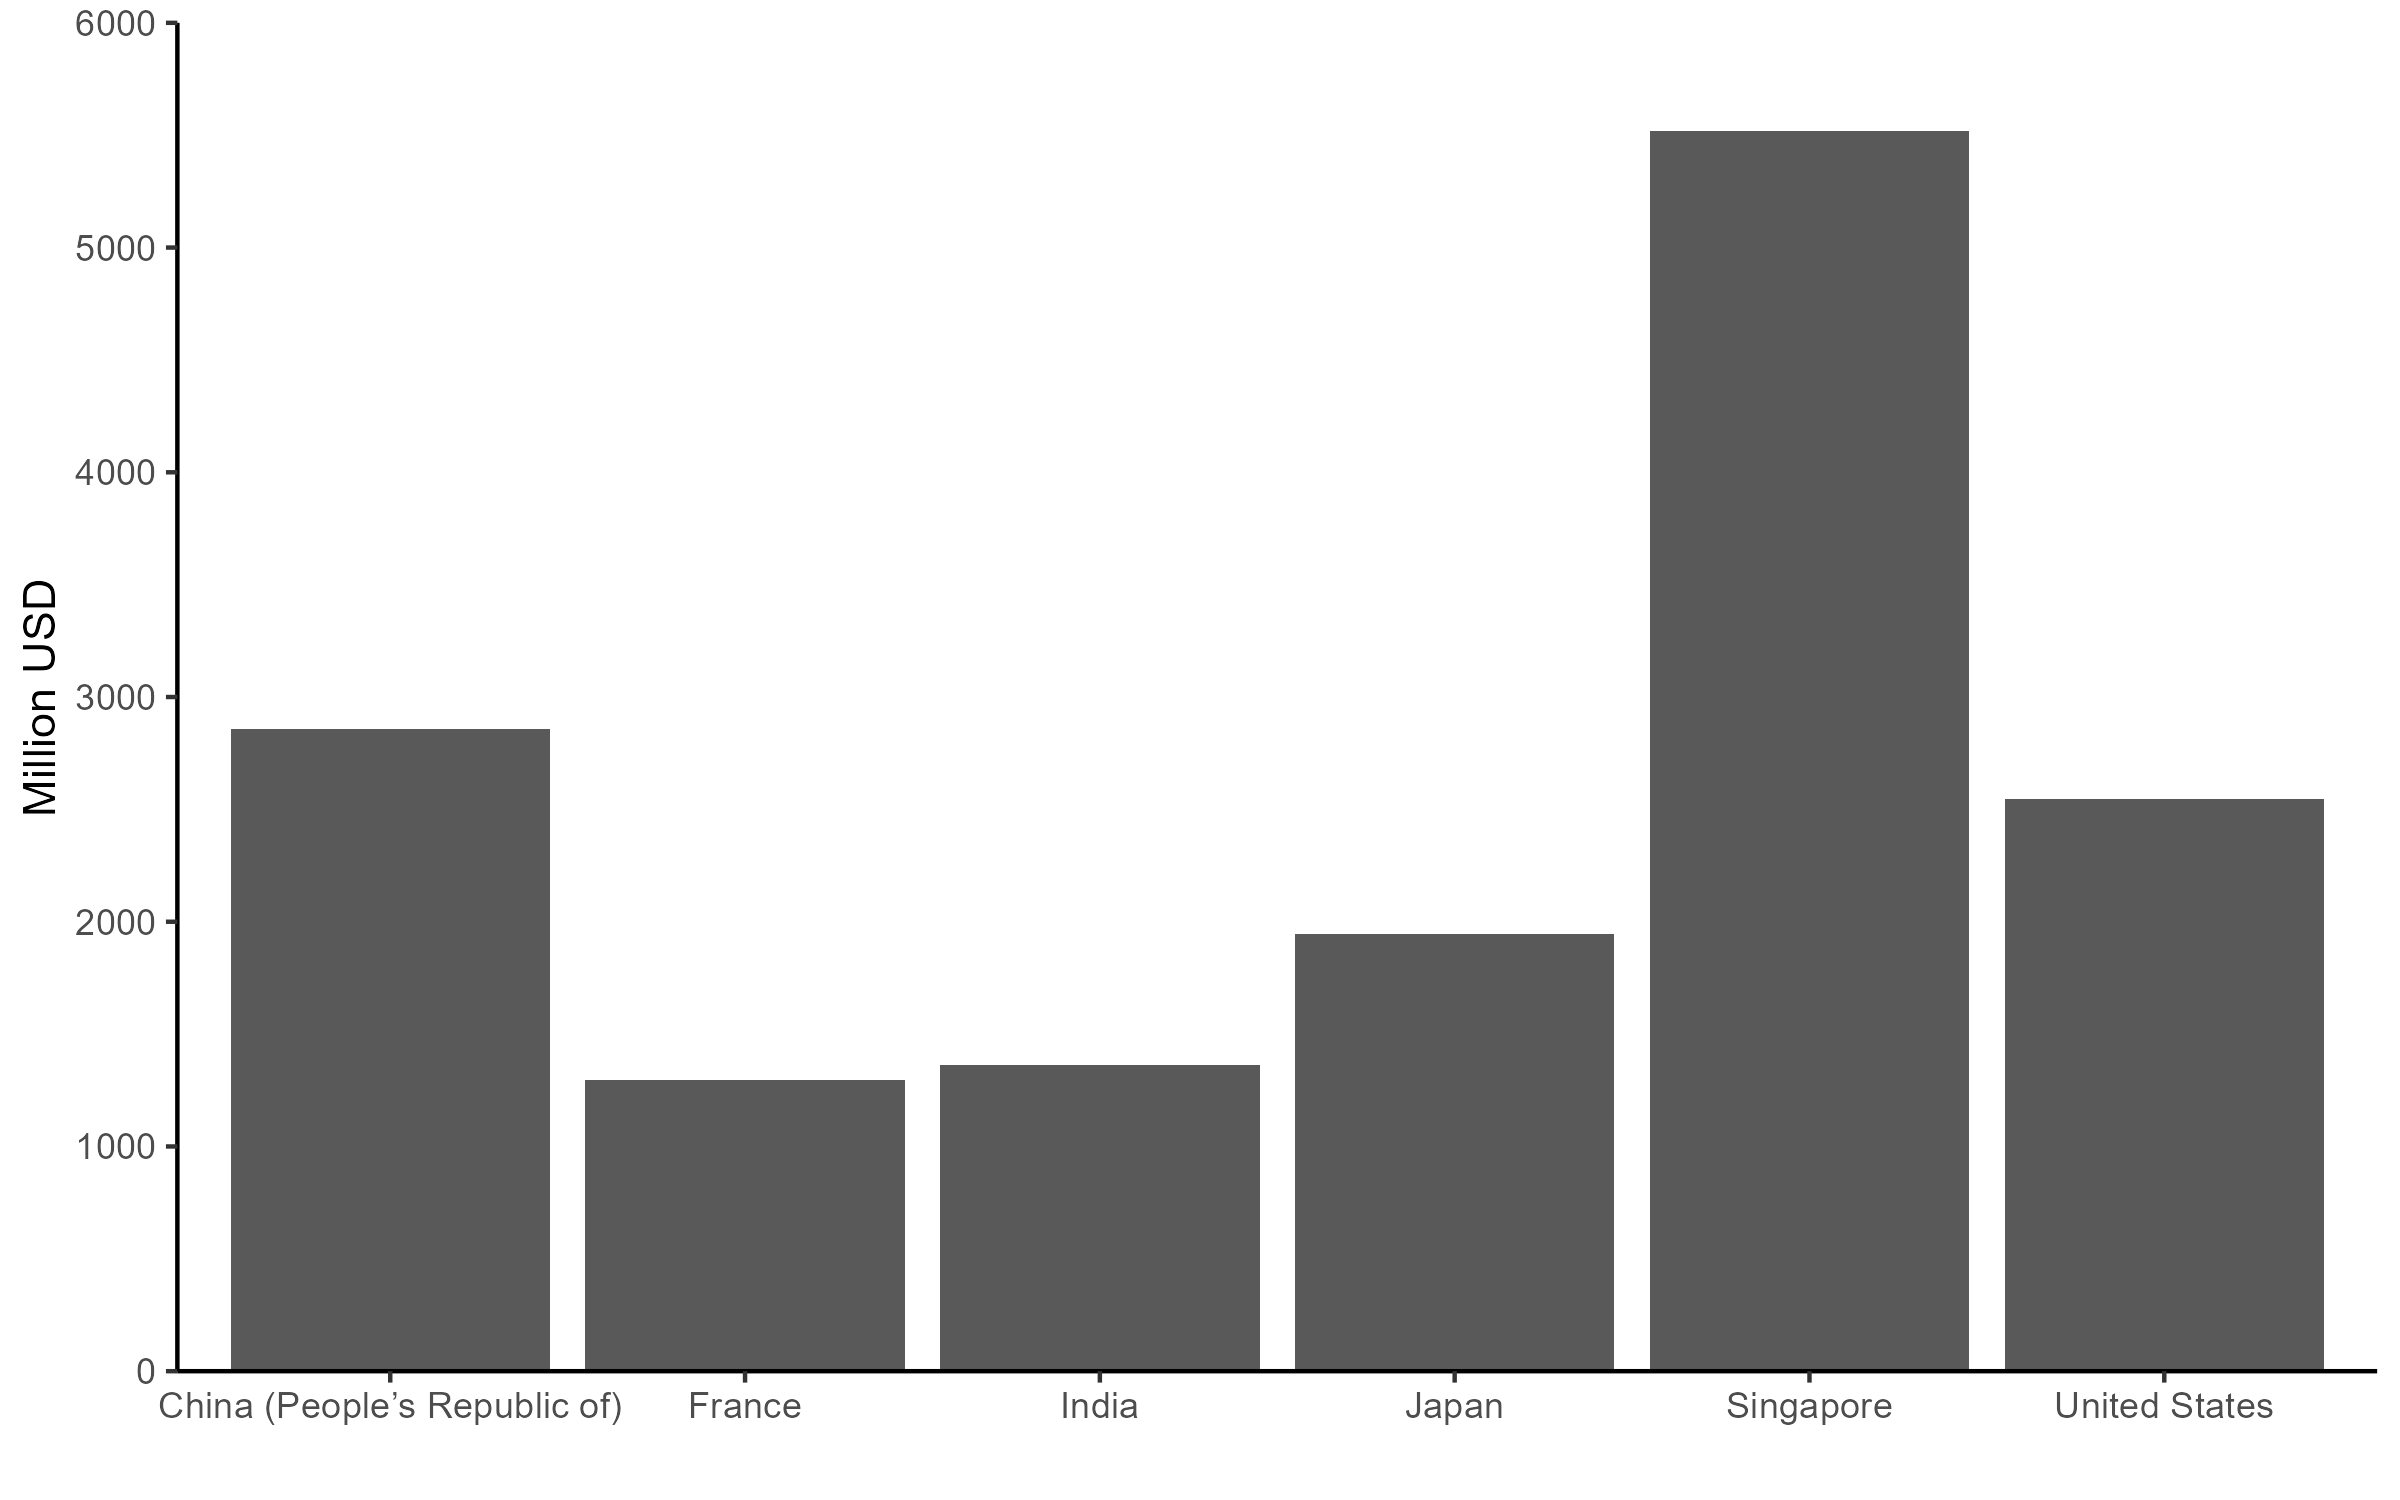
\includegraphics{plot/allcm.png}

}

\subcaption{\label{fig-CM}Indonesia's exports by partner, 2021}

\end{minipage}%
\newline
\begin{minipage}{0.50\linewidth}

\centering{

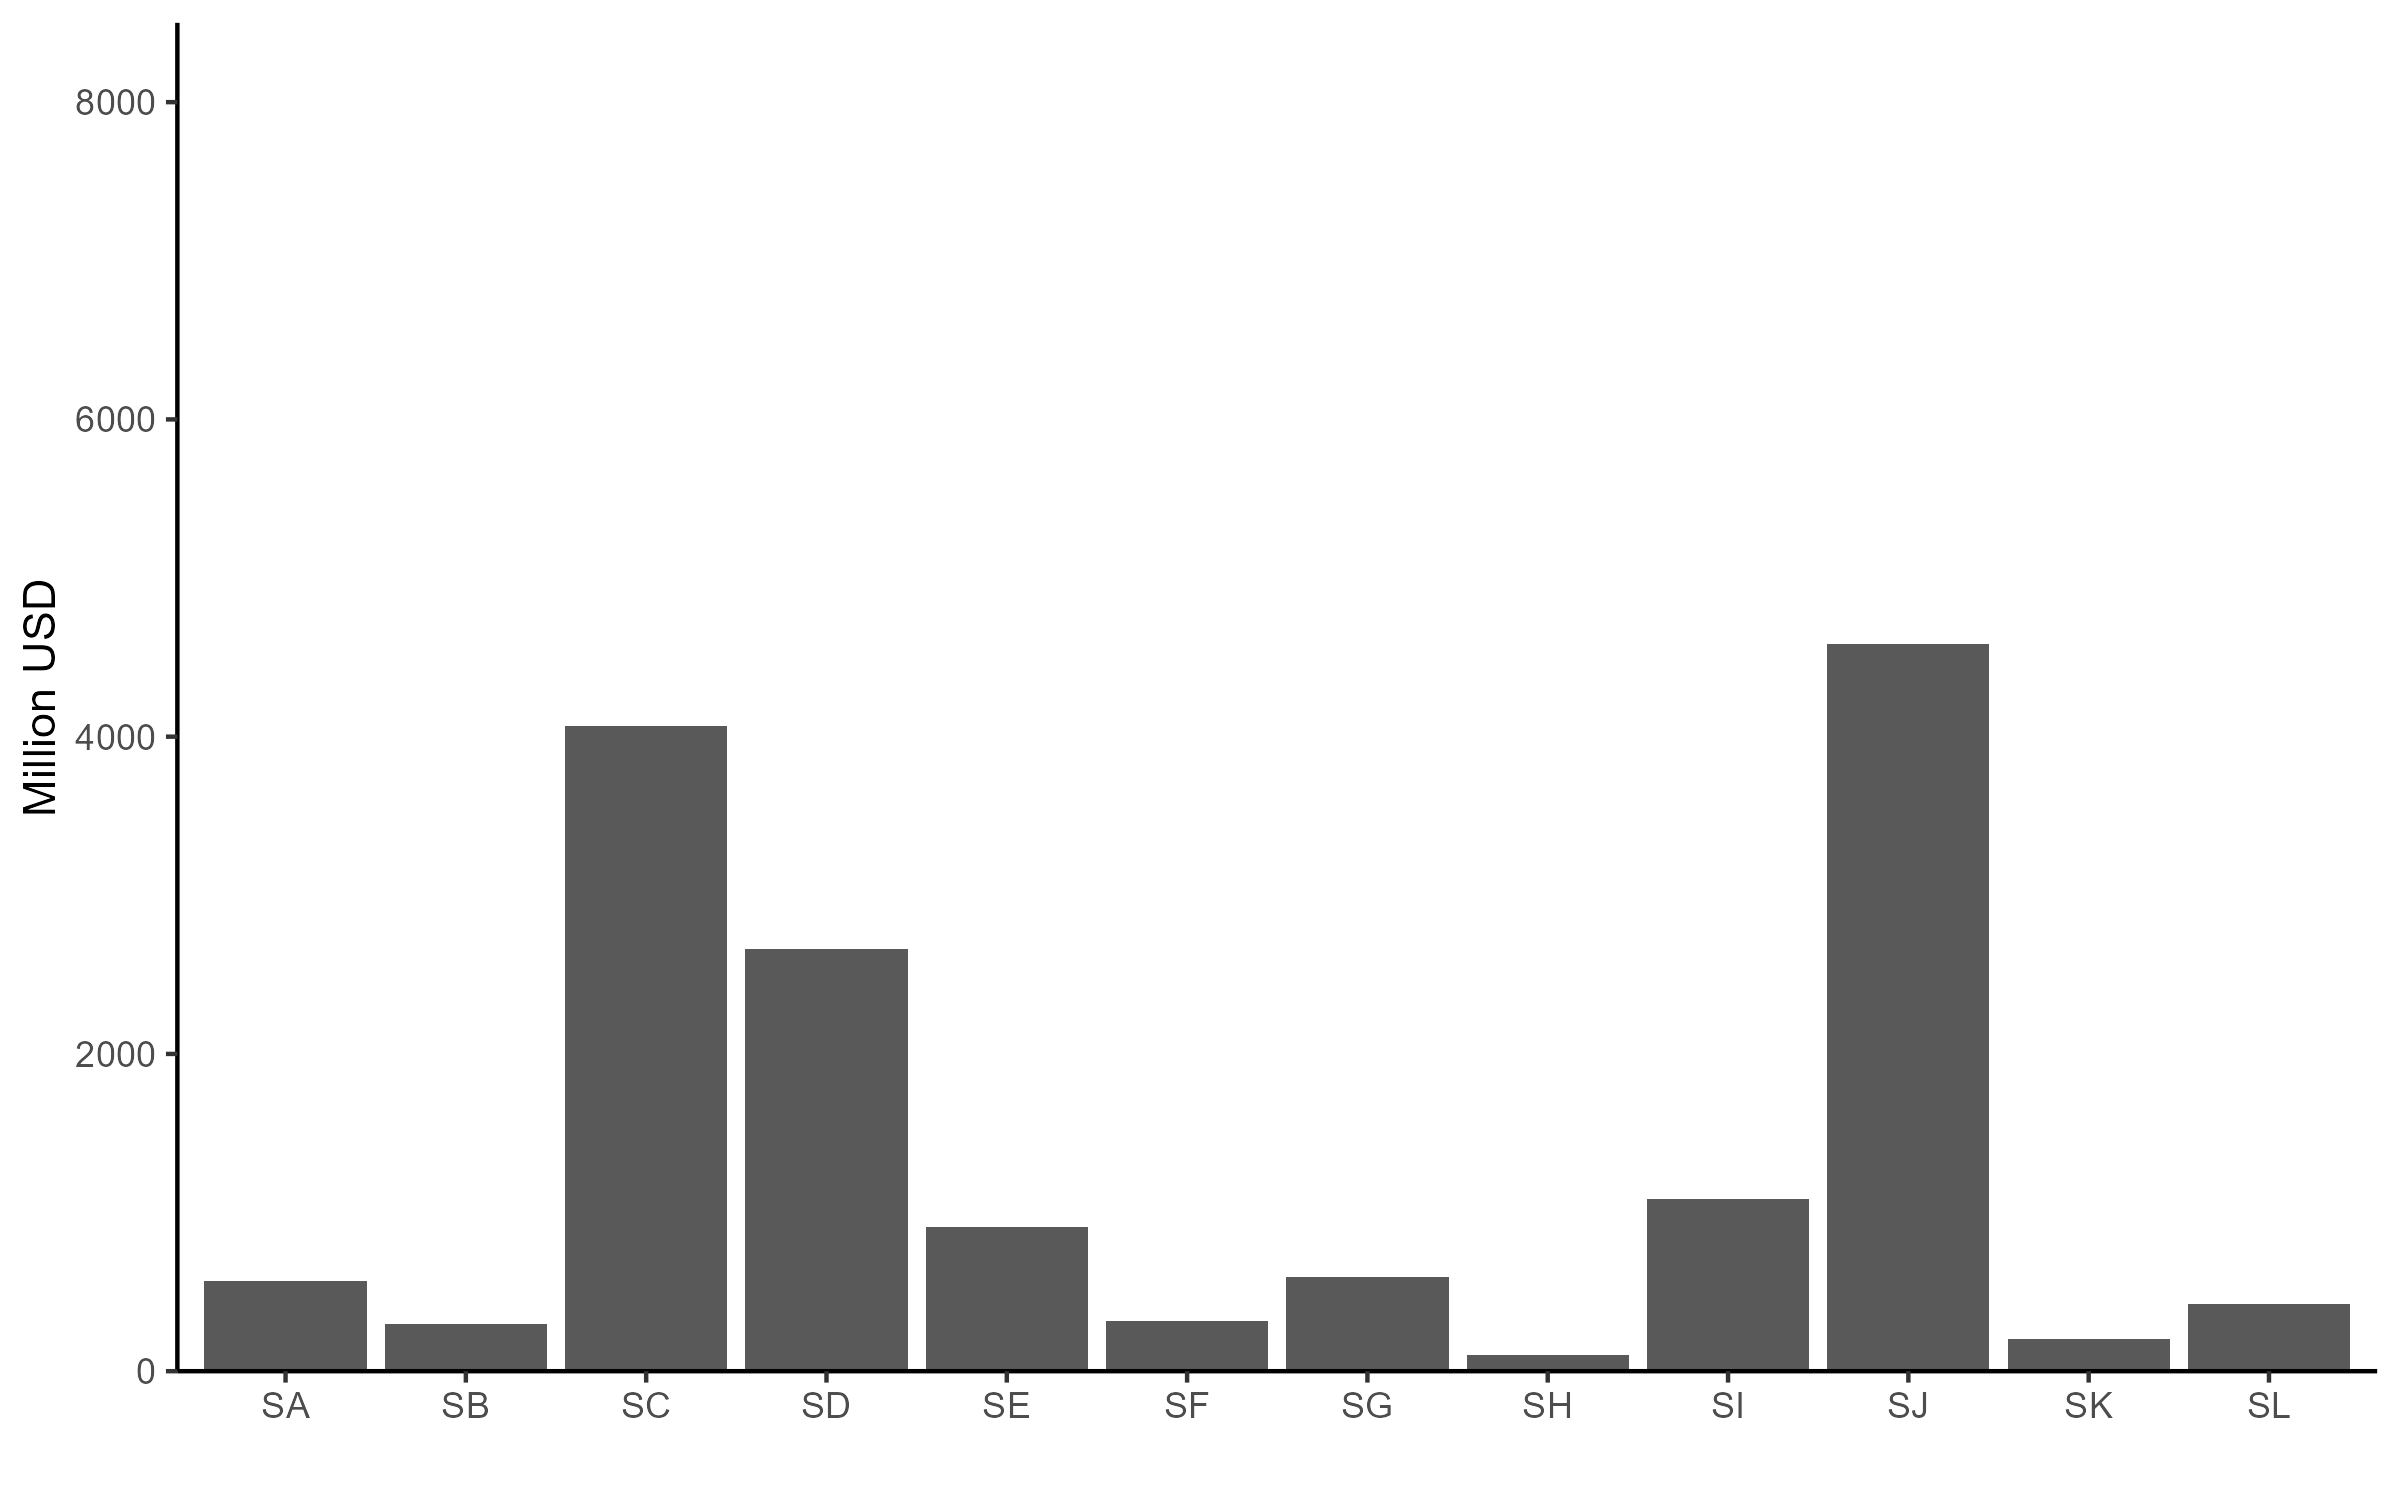
\includegraphics{plot/allsx.png}

}

\subcaption{\label{fig-SX}Indonesia's exports by sector, 2021}

\end{minipage}%
%
\begin{minipage}{0.50\linewidth}

\centering{

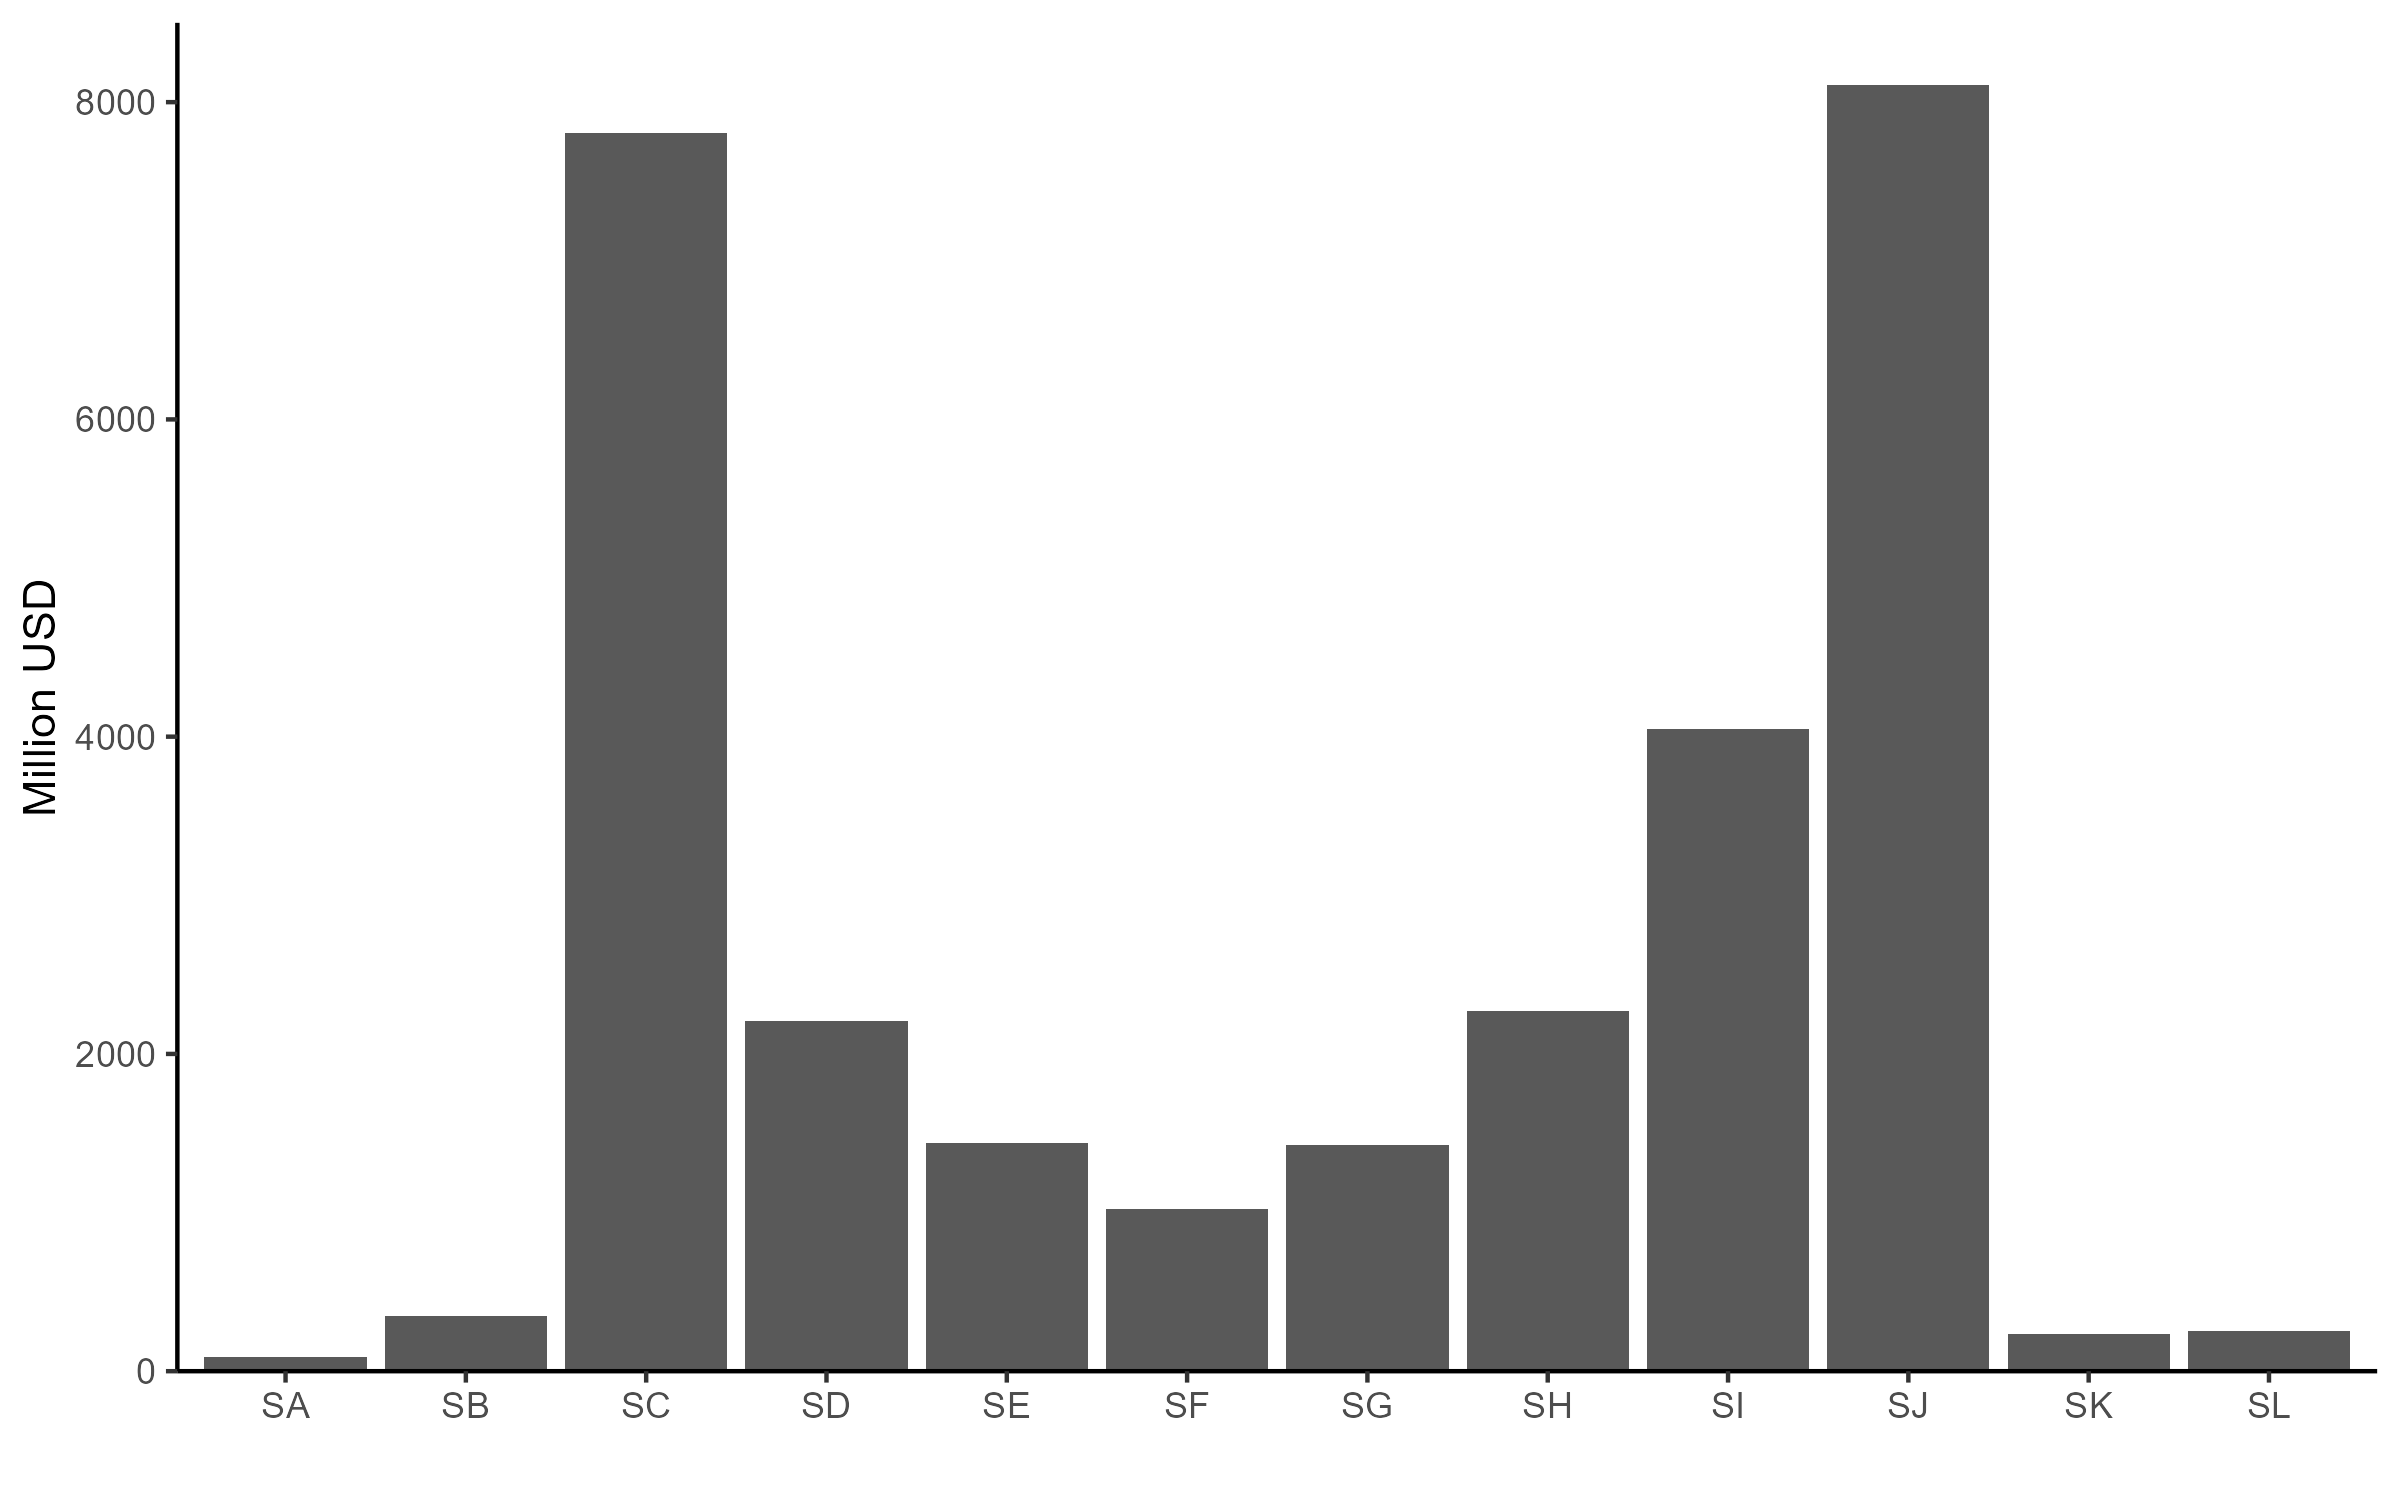
\includegraphics{plot/allsm.png}

}

\subcaption{\label{fig-SM}Indonesia's imports by sector, 2021}

\end{minipage}%

\caption{\label{fig-S}Indonesia's total services trade by categories,
2021}

\end{figure}%

We then focuses on Indonesia's four most important services. These are
transport (SC), travel (SD), ICT services (SI) and other business
services (SJ). Other business services includes consulting management,
research and development, and trade-related services (Liberatore et al.
2021). We look at top 6 partners in these sectors annually from
2005-2021 as existed in BaTIS, which can be seen in Figure~\ref{fig-X}
(exports) and Figure~\ref{fig-M} (imports). Some countries change
positions in these top 6 from time to time. A sudden miss of a country
does not mean it stops trading with Indonesia, it's just they are
removed from the top 6.

\begin{figure}

\begin{minipage}{0.50\linewidth}

\centering{

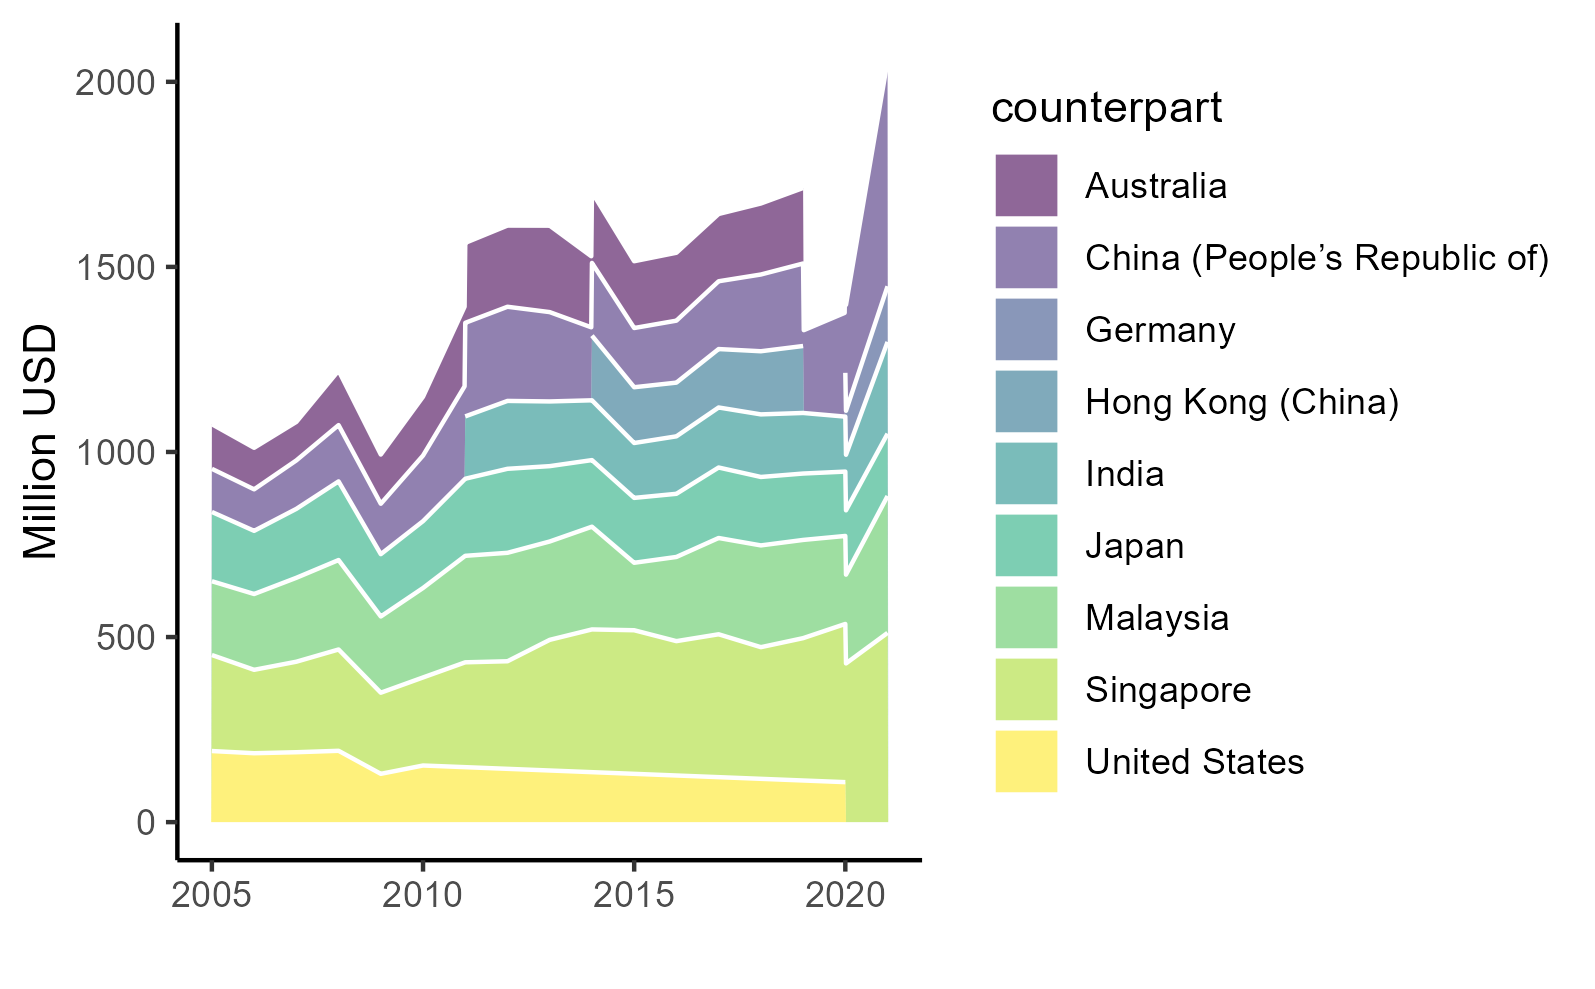
\includegraphics{plot/SCEX.png}

}

\subcaption{\label{fig-SCX}Transport}

\end{minipage}%
%
\begin{minipage}{0.50\linewidth}

\centering{

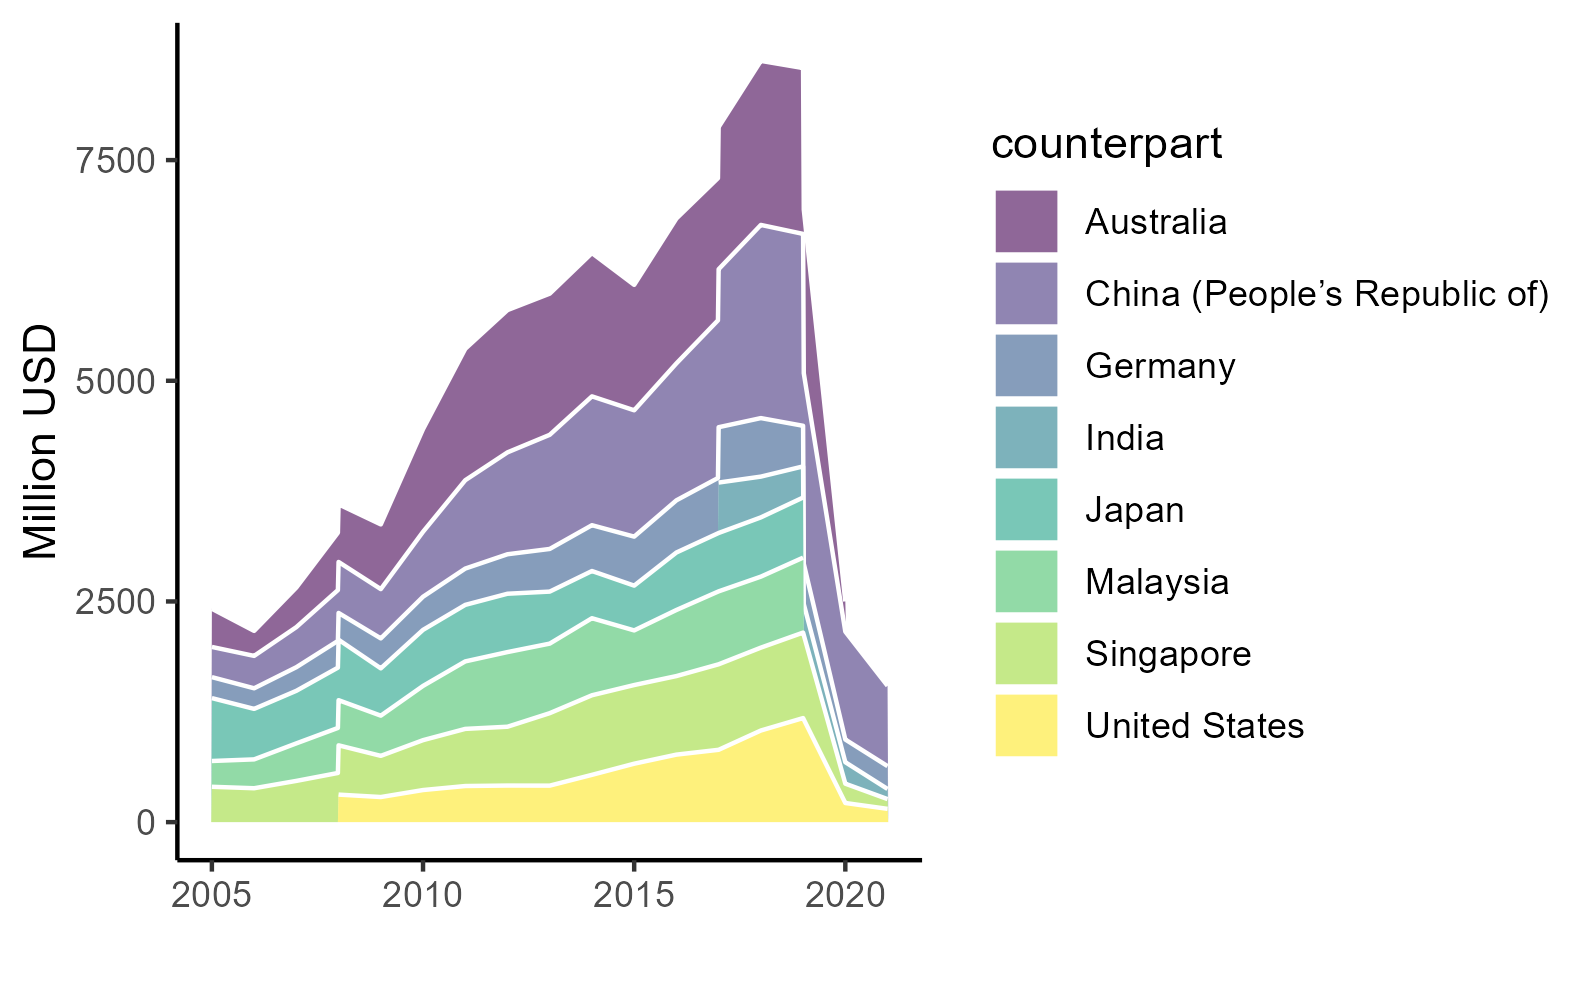
\includegraphics{plot/SDEX.png}

}

\subcaption{\label{fig-SDX}Travel}

\end{minipage}%
\newline
\begin{minipage}{0.50\linewidth}

\centering{

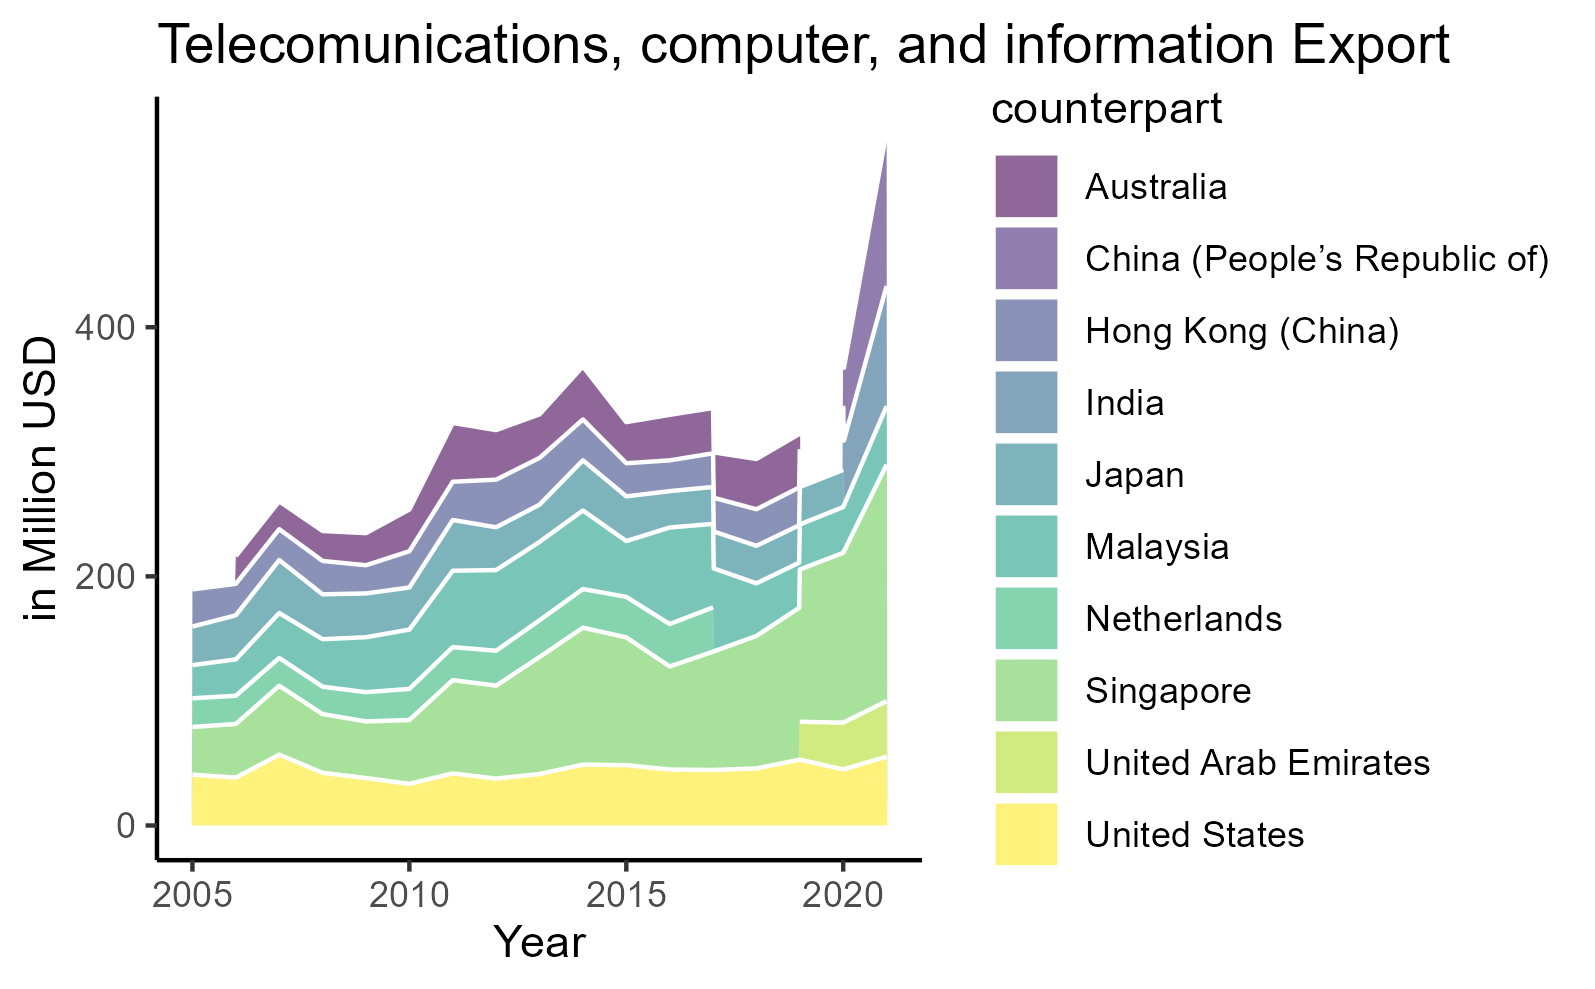
\includegraphics{plot/SIEX.png}

}

\subcaption{\label{fig-SIX}ICT services}

\end{minipage}%
%
\begin{minipage}{0.50\linewidth}

\centering{

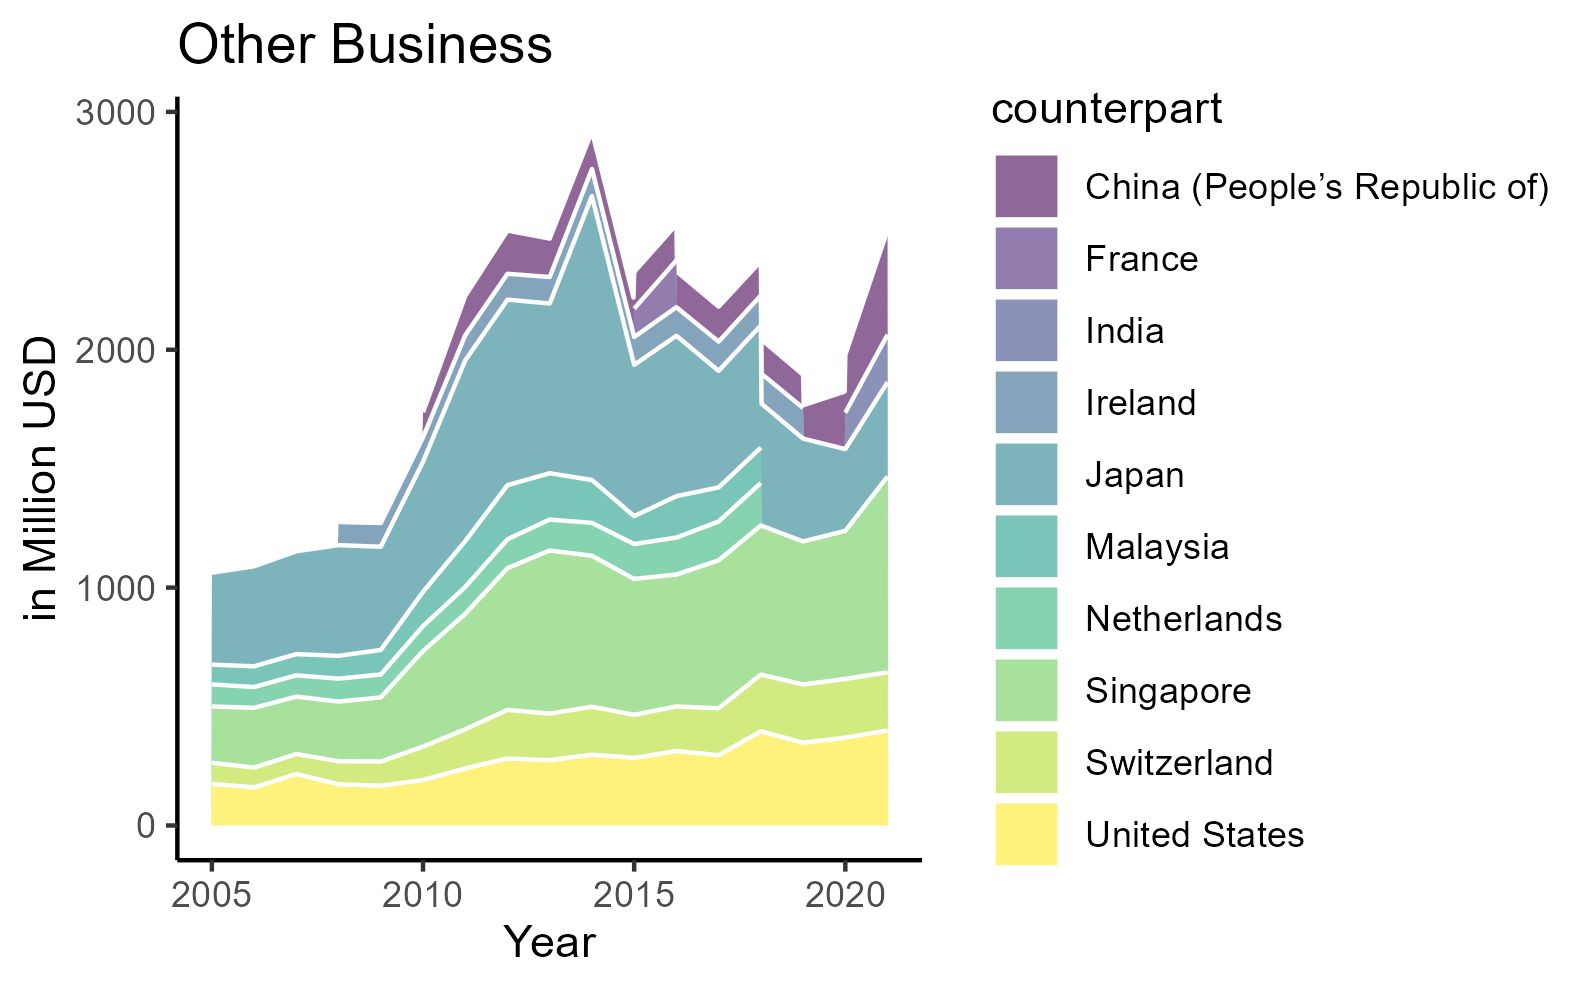
\includegraphics{plot/SJEX.png}

}

\subcaption{\label{fig-SJX}Other business services}

\end{minipage}%

\caption{\label{fig-X}Indonesia's top 6 exporter destinations to 4
categories, 2005-2021}

\end{figure}%

\begin{figure}

\begin{minipage}{0.50\linewidth}

\centering{

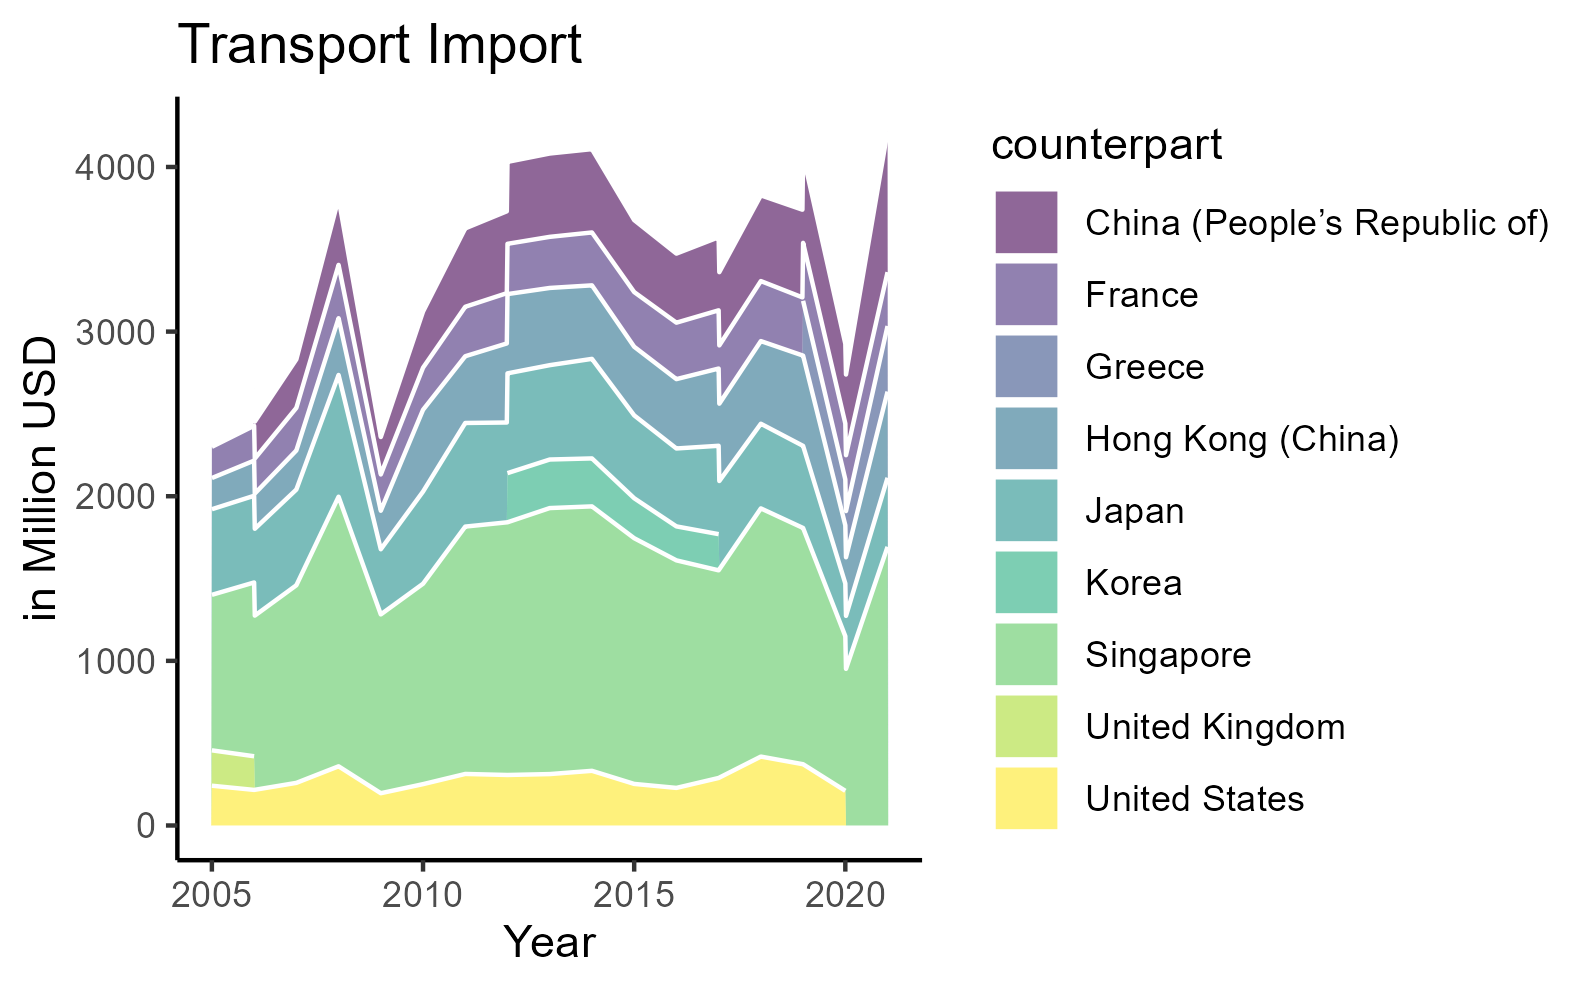
\includegraphics{plot/SCIM.png}

}

\subcaption{\label{fig-SCM}Transport}

\end{minipage}%
%
\begin{minipage}{0.50\linewidth}

\centering{

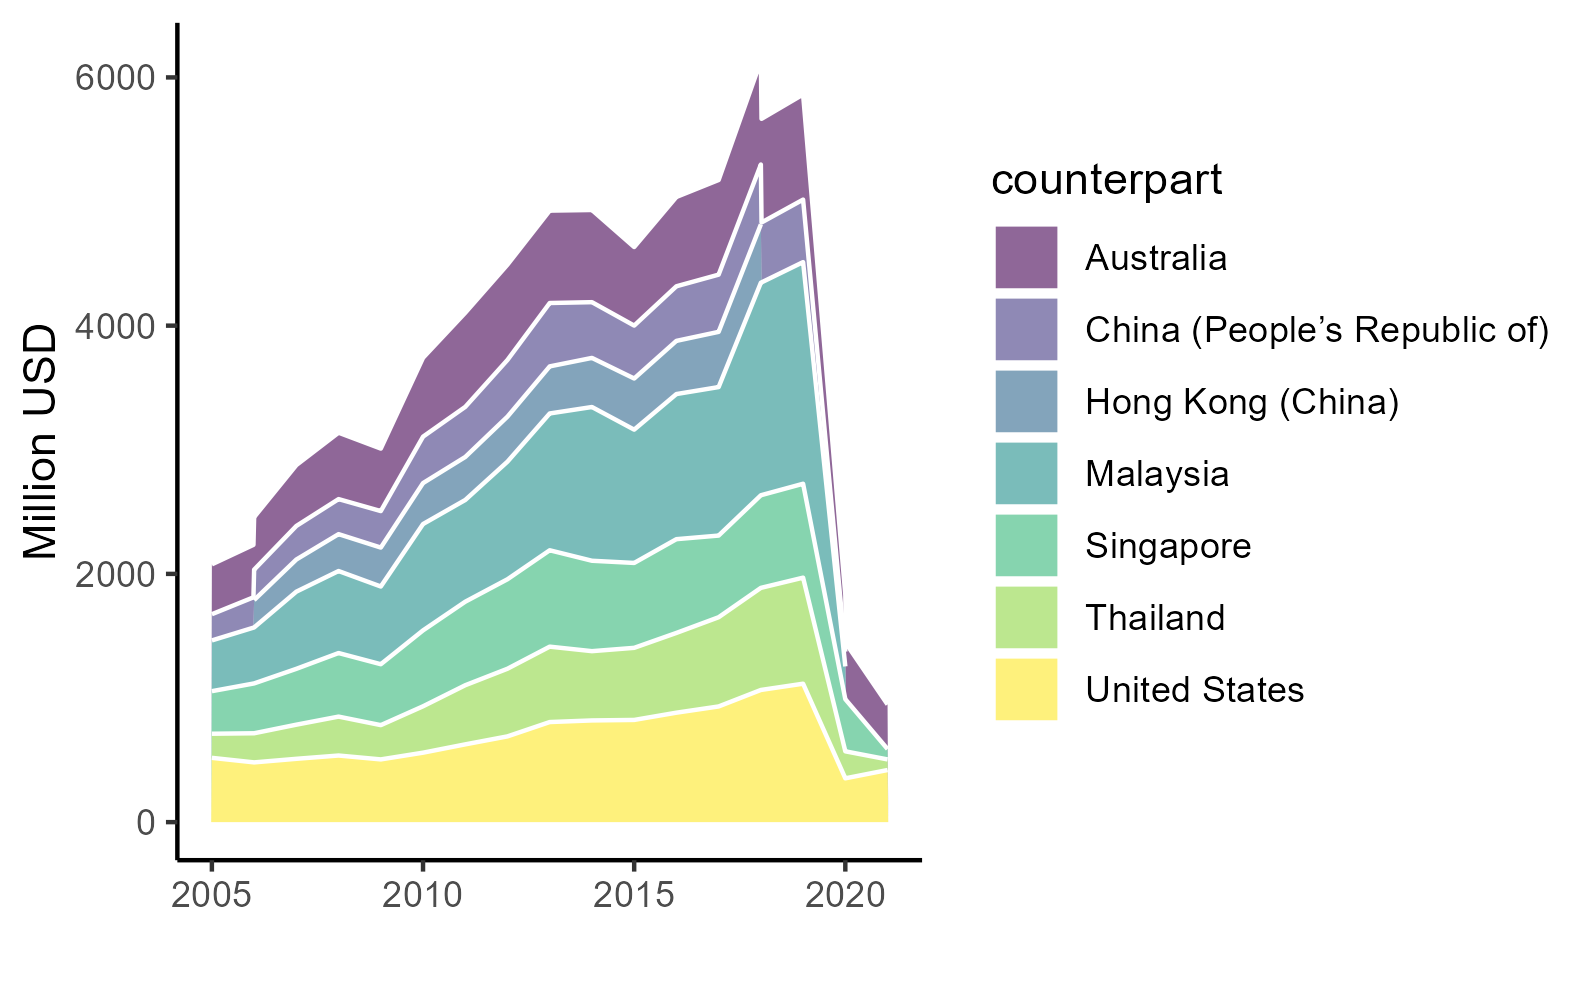
\includegraphics{plot/SDIM.png}

}

\subcaption{\label{fig-SDM}Travel}

\end{minipage}%
\newline
\begin{minipage}{0.50\linewidth}

\centering{

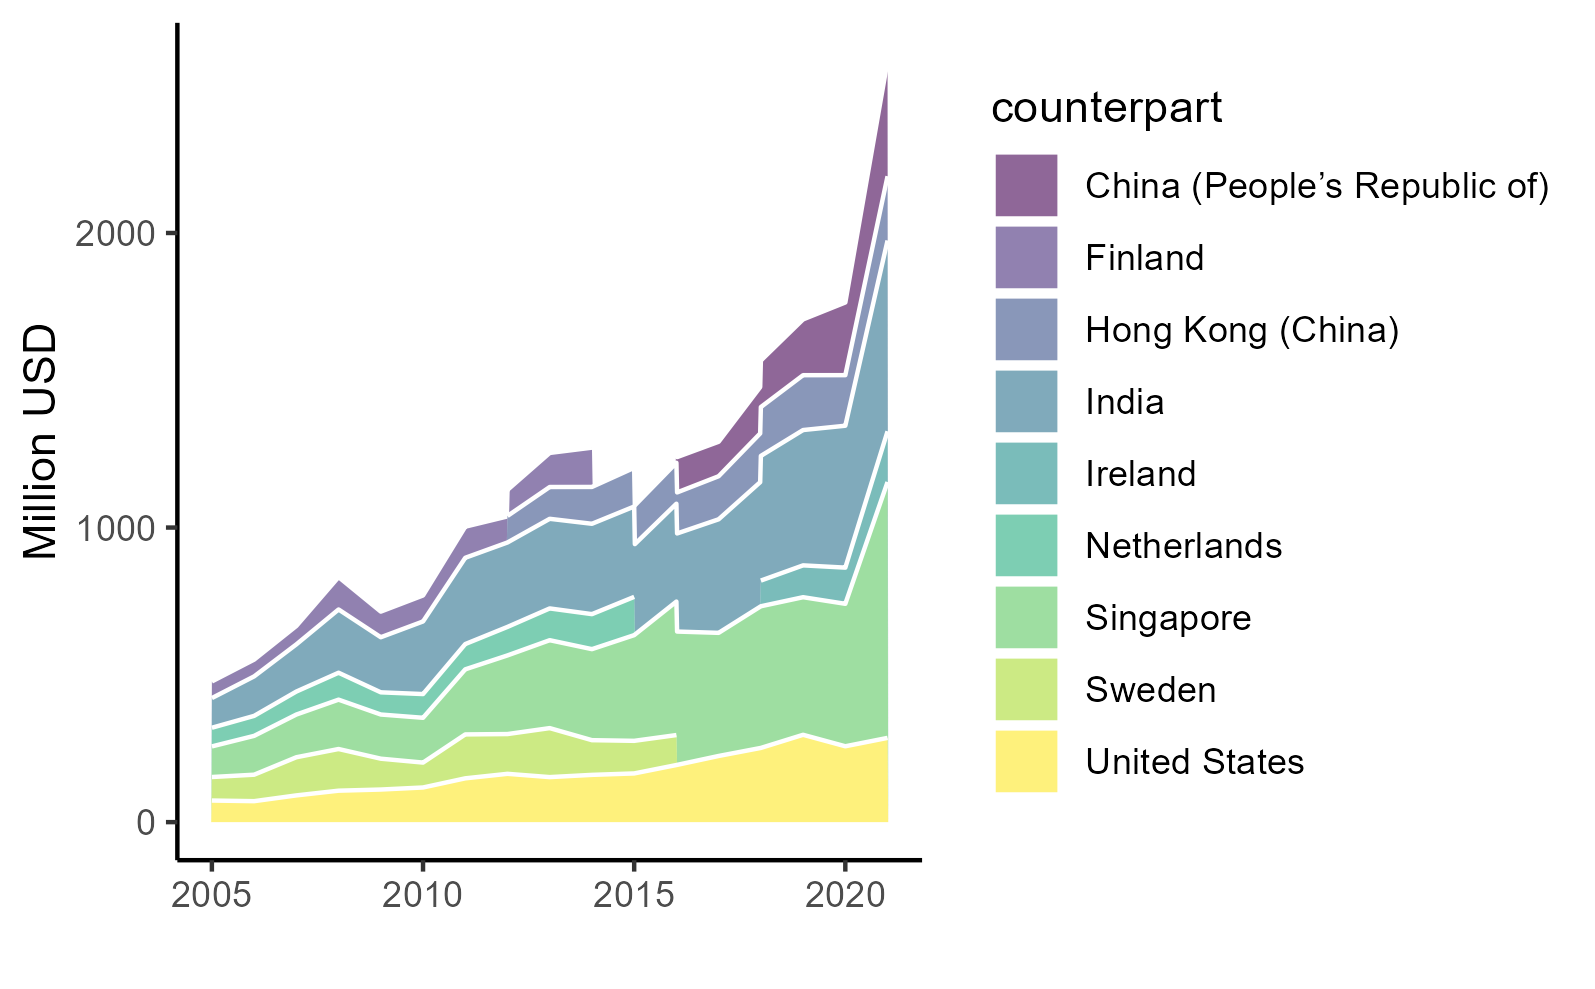
\includegraphics{plot/SIIM.png}

}

\subcaption{\label{fig-SIM}ICT services}

\end{minipage}%
%
\begin{minipage}{0.50\linewidth}

\centering{

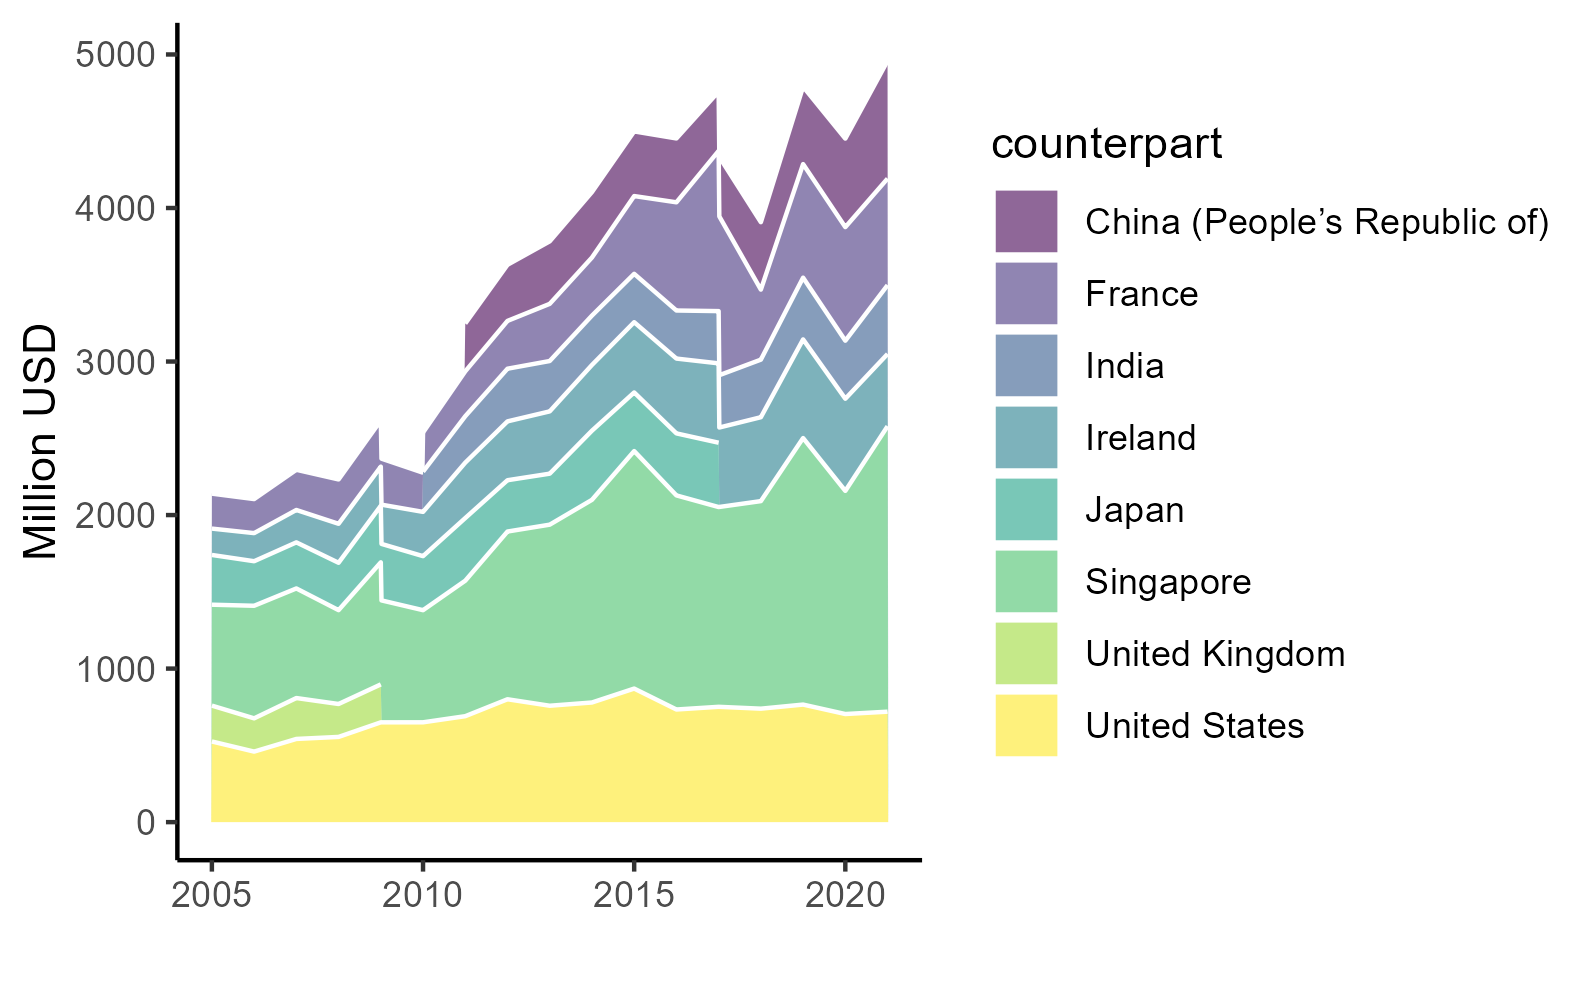
\includegraphics{plot/SJIM.png}

}

\subcaption{\label{fig-SJM}Other business services}

\end{minipage}%

\caption{\label{fig-M}Indonesia's top 6 import sources in 4 categories,
2005-2021}

\end{figure}%

Immediately, Figure~\ref{fig-X} and Figure~\ref{fig-M} show significant
changes happened in 2020 and 2021, which corroborates the aggregated
data in Figure~\ref{fig-1}. This is likely due to the COVID-19 pandemic
that restrict movement of people.

This shock, however, affects differently between these four sectors. The
transportation sector decrease quite significantly in 2020, but
recovered relatively quickly in 2021. The impact in the business
services is milder compared to the transportation sector. Meanwhile, we
see a significant drop in travel services and have not recovered since.
Meanwhile, ICT services are the winner here, with the top 6 partners
experience significant increase in both 2020 and 2021.

Singapore is indeed important in both export and import. Singapore
relationship with Indonesia in trade in services dwarves the rest, and
this is true for almost all sectors. Travel export is slightly the
exception. China and Australia dominates as destinations for Indonesian
travel export. In Indonesia, most travel exports comes mainly from
tourism. Indeed, tourism is Indonesia's main services export. Pre-2020,
travel services from 6 top exporters far dominates the other 3
categories. Pandemic punishes travel exports more than other sectors and
it affects Indonesia's overall balance of trade in services.

Overall, countries important for Indonesia in trade in services is not
significantly different from trade in goods. Singapore leads, but there
are also the US, some EU countries, and other RCEP member states. Trade
agreements play a huge role in improving trade in services. Measures
that affects movement of natural persons, and other non-tariff measures
like computing requirement and investment list are crucial as trade in
services can be done in 4 different modes that got affected by these
rules.

Typically, overseeing trade in services and regulatory environment
required to increase flow of trade in services are more challenging than
trade in goods. In Indonesia, these regulations are often oversaw by
different Ministries, and typically discussed separately from other
sectors or trade negotiations (Magiera 2011; Lindblad 2015). Discussing
regulatory environment to improve trade in services would require
coordination which is costly compared to trade in goods.

For example, easing tourism visa requirement typically conducted
unilaterally with no consultation with other ministries or any
agreements. These kinds of regulation relies more on each Ministers than
agreement mechanisms. While IJEPA doesn't seem to affect trade in
services much between Indonesia and Japan (Syahputri and Gupta 2024),
IACEPA between Indonesia and Australia seems to improve Australian
services export through investment in university and hospital.

More importantly, easing services trade may benefit Indonesia through
the third unbundling mechanisms. Many exported services are
skill-intensive products, which arguably not Indonesia's main strength.
If these services are important in a production chain of final goods,
then outsourcing services production (e.g., design and research) will
benefit Indonesian manufacturing. The next section explores an
indicative evidence toward this argument.

\subsubsection{Manufacturing}\label{manufacturing}

\paragraph{ICIO Panel regression}\label{icio-panel-regression}

We first turn to our panel regression shown in Equation~\ref{eq-2}. As
discussed, we run a total 12 regressions divided into two tables.
Table~\ref{tbl-regv} shows results for log of value added as the
dependent variable, while \textbf{?@tbl-rego} is on output. Each table
has 6 regressions, which the first column show a result from all
countries combined and the rest are from each countries.

\begin{figure}

\begin{minipage}{0.50\linewidth}

\begin{figure}[H]

\centering{

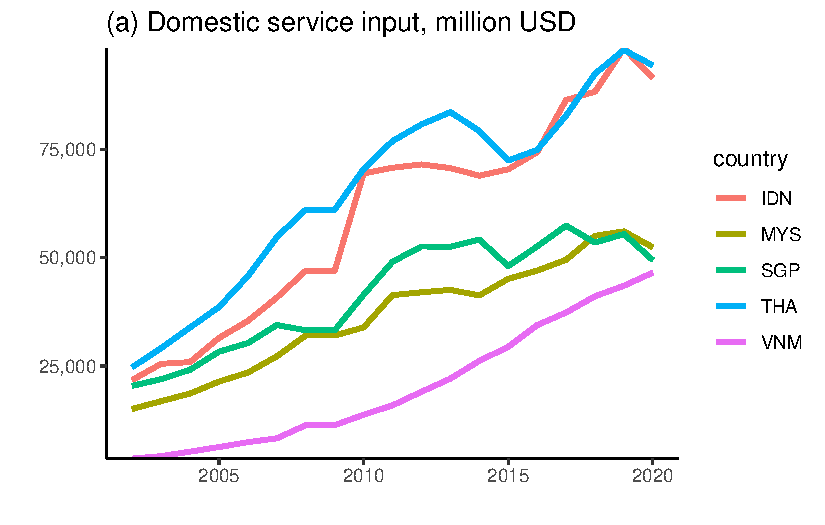
\includegraphics{services_document_files/figure-pdf/fig-ser-1.pdf}

}

\caption{\label{fig-ser-1}}

\end{figure}%

\end{minipage}%
%
\begin{minipage}{0.50\linewidth}

\begin{figure}[H]

\centering{

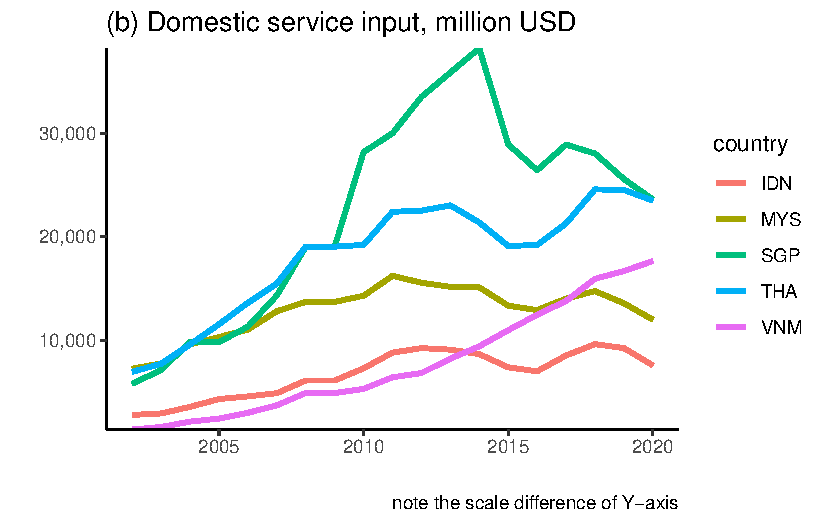
\includegraphics{services_document_files/figure-pdf/fig-ser-2.pdf}

}

\caption{\label{fig-ser-2}}

\end{figure}%

\end{minipage}%

\end{figure}%

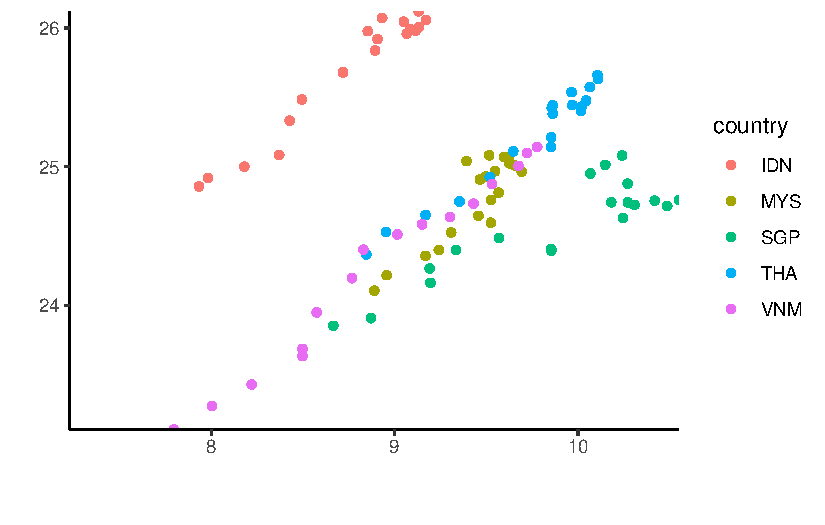
\includegraphics{services_document_files/figure-pdf/unnamed-chunk-8-1.pdf}

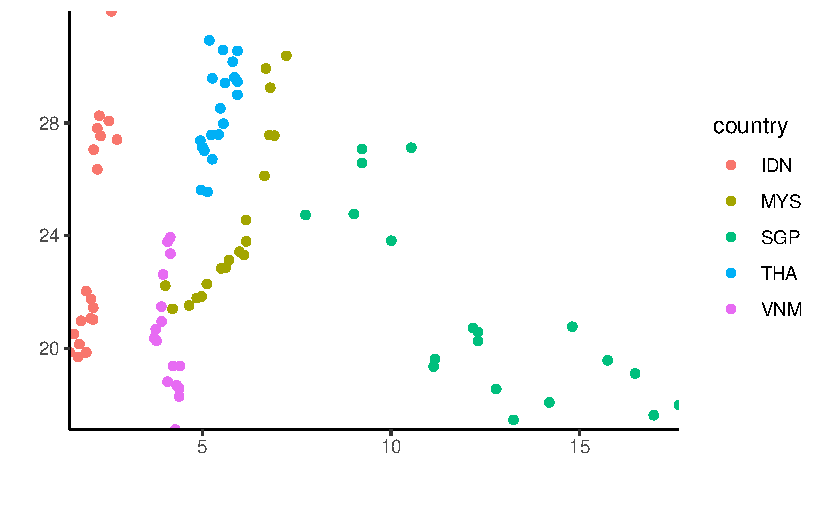
\includegraphics{services_document_files/figure-pdf/unnamed-chunk-8-2.pdf}

```

\begin{table}

\caption{\label{tbl-regv}Panel regression of log manufacturing value
added}

\centering{

\centering
\begin{talltblr}[         %% tabularray outer open
entry=none,label=none,
note{}={+ p < 0.1, * p < 0.05, ** p < 0.01, *** p < 0.001},
]                     %% tabularray outer close
{                     %% tabularray inner open
colspec={Q[]Q[]Q[]Q[]},
column{1}={halign=l,},
column{2}={halign=c,},
column{3}={halign=c,},
column{4}={halign=c,},
hline{8}={1,2,3,4}{solid, 0.05em, black},
}                     %% tabularray inner close
\toprule
& OLS & FE & TWFE \\ \midrule %% TinyTableHeader
(Intercept) & \num{15.772}*** &                &                \\
& (\num{0.313})   &                &                \\
lfs         & \num{-0.467}*** & \num{0.154}   & \num{0.157}   \\
& (\num{0.034})   & (\num{0.140}) & (\num{0.139}) \\
lds         & \num{1.278}***  & \num{0.783}** & \num{0.800}** \\
& (\num{0.036})   & (\num{0.141}) & (\num{0.131}) \\
Num.Obs.    & \num{92}        & \num{92}      & \num{92}      \\
R2          & \num{0.939}     & \num{0.985}   & \num{0.987}   \\
R2 Within   &                  & \num{0.966}   & \num{0.806}   \\
\bottomrule
\end{talltblr}

}

\end{table}%

First, we look at value added. We can see from Table~\ref{tbl-regv} that
domestic services are generally correlates with domestic manufacturing
value added. However, foreign value added does not seem to be important
in the domestic value added of manufacturing. Vietnam is the exception,
where foreign services seem to move together with domestic value added.

\begin{table}

\caption{\label{tbl-regvv}Panel regression of log manufacturing value
added}

\centering{

\centering
\begin{talltblr}[         %% tabularray outer open
entry=none,label=none,
note{}={+ p < 0.1, * p < 0.05, ** p < 0.01, *** p < 0.001},
]                     %% tabularray outer close
{                     %% tabularray inner open
colspec={Q[]Q[]Q[]Q[]},
column{1}={halign=l,},
column{2}={halign=c,},
column{3}={halign=c,},
column{4}={halign=c,},
hline{8}={1,2,3,4}{solid, 0.05em, black},
}                     %% tabularray inner close
\toprule
& RE & FE & TWFE \\ \midrule %% TinyTableHeader
(Intercept) & \num{21.476}*** &                &                \\
& (\num{1.590})   &                &                \\
psfs        & \num{-0.501}*** & \num{-0.341}  & \num{-0.160}  \\
& (\num{0.138})   & (\num{0.582}) & (\num{0.335}) \\
psds        & \num{0.018}**   & \num{-0.029}  & \num{-0.011}  \\
& (\num{0.007})   & (\num{0.015}) & (\num{0.039}) \\
Num.Obs.    & \num{92}        & \num{92}      & \num{92}      \\
R2          & \num{0.131}     & \num{0.522}   & \num{0.775}   \\
R2 Within   &                  & \num{0.062}   & \num{0.022}   \\
\bottomrule
\end{talltblr}

}

\end{table}%

\paragraph{ARDL results}\label{ardl-results}

We complement previous analysis with more macro, less structured
approach. We test whether services import and manufacturing export and
output moves together. Figure~\ref{fig-idn} shows data we use.
Manufacturing GDP is omitted for scaling reason, but we can see the vast
difference between merchandise trade and services trade during the
pandemic in 2020. While we use internet and computer application
services more during the pandemic, the huge drop in travels visually
dominates Indonesia's import services. In fact, it is because we can
have digital presence that traveling abroad is less needed even as
restriction eases.

\begin{figure}

\centering{

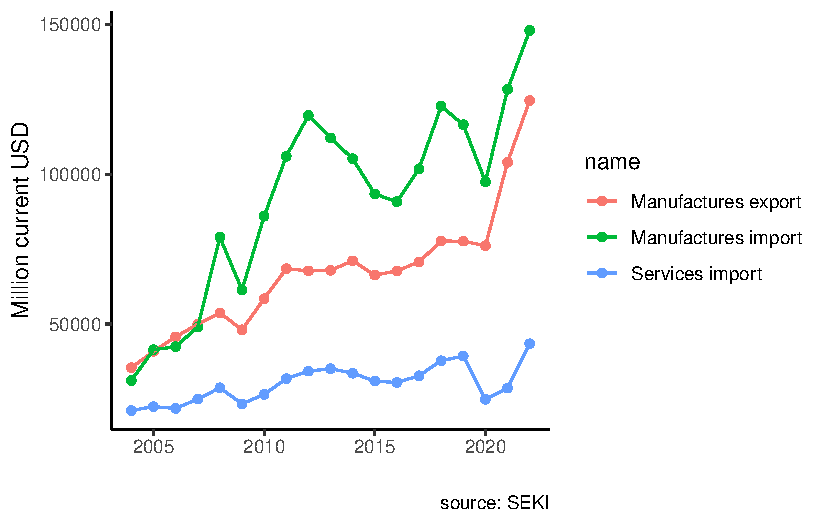
\includegraphics{services_document_files/figure-pdf/fig-idn-1.pdf}

}

\caption{\label{fig-idn}Indonesian trade dynamics}

\end{figure}%

The log version of variables in Figure~\ref{fig-idn} is used for the
regression, along with log of manufacturing GDP. Summary statistics are
presented in \textbf{?@tbl-sum2}.

Results from executing Equation~\ref{eq-3} is shown in
Table~\ref{tbl-2}. There are four column, with the first two use log
manufactures exports as the left hand-side variable while the latter two
uses log manufacturing GDP. \texttt{ARDL(1,0,0)} is used for the first
column and \texttt{ARDL(1,1,1)} is used for the second column of each,
as discussed in the previous section.

\begin{table}

\caption{\label{tbl-2}ARDL results on four specifications}

\centering{

\centering
\begin{talltblr}[         %% tabularray outer open
entry=none,label=none,
note{}={+ p < 0.1, * p < 0.05, ** p < 0.01, *** p < 0.001},
]                     %% tabularray outer close
{                     %% tabularray inner open
colspec={Q[]Q[]Q[]Q[]Q[]},
column{1}={halign=l,},
column{2}={halign=c,},
column{3}={halign=c,},
column{4}={halign=c,},
column{5}={halign=c,},
hline{16}={1,2,3,4,5}{solid, 0.05em, black},
}                     %% tabularray inner close
\toprule
& Export 1 & Export 2 & GDP 1 & GDP 2 \\ \midrule %% TinyTableHeader
(Intercept) & \num{0.704}   & \num{1.354}+   & \num{0.112}    & \num{0.243}+   \\
& (\num{0.724}) & (\num{0.692})  & (\num{0.127})  & (\num{0.128})  \\
L(exM, 1)   & \num{0.676}** & \num{1.135}*** &                 &                 \\
& (\num{0.222}) & (\num{0.177})  &                 &                 \\
imM         & \num{0.273}   & \num{0.307}*   & \num{-0.003}   & \num{-0.023}   \\
& (\num{0.184}) & (\num{0.127})  & (\num{0.020})  & (\num{0.022})  \\
imSev       & \num{-0.106}  & \num{-0.130}   & \num{0.098}**  & \num{0.110}*** \\
& (\num{0.247}) & (\num{0.146})  & (\num{0.029})  & (\num{0.024})  \\
L(imM, 1)   &                & \num{-0.151}   &                 & \num{0.031}    \\
&                & (\num{0.166})  &                 & (\num{0.023})  \\
L(imSev, 1) &                & \num{-0.485}*  &                 & \num{-0.083}*  \\
&                & (\num{0.182})  &                 & (\num{0.030})  \\
L(pdb, 1)   &                &                 & \num{0.917}*** & \num{0.938}*** \\
&                &                 & (\num{0.024})  & (\num{0.022})  \\
Num.Obs.    & \num{18}      & \num{18}       & \num{18}       & \num{18}       \\
R2          & \num{0.881}   & \num{0.967}    & \num{0.997}    & \num{0.998}    \\
Log.Lik.    & \num{32.291}  & \num{43.772}   & \num{70.818}   & \num{76.085}   \\
RMSE        & \num{0.04}    & \num{0.02}     & \num{0.00}     & \num{0.00}     \\
\bottomrule
\end{talltblr}

}

\end{table}%

Table~\ref{tbl-2} shows that Indonesia's current import service does not
seem to contribute much to the country's manufacturing export. The
coefficient is found to be negative but not different from zero. This
does not seem to be surprising since it corroborates findings in
Table~\ref{tbl-regv} and Table~\ref{tbl-regv}. Additionally, Indonesian
firms does not seem to have much in house services to begin with, and
those who do are only a small fraction of very productive firms (Hing
and Thangavelu 2023).

For manufacturing output, however, we find that import services
correlates significantly with manufacturing output. A 1\% increase in
service import correlates with a 0.1\% increase in manufacturing output.
This correlation may stem from imported goods import. That is,
Indonesian manufacturers requires various imported intermediate inputs.
Therefore, increasing production requires importing various goods,
increasing the use of transport service, which is dominated by foreign
firms. This explains why imported service does not correlate with
manufacturing export, and why manufactures import correlates positively
with exports.

This findings seem to suggests that Indonesian manufacturing use
services mostly for international trade purposes. Since transport
dominates Indonesia's trade in services, it seems to suggest that
Indonesian manufacturing does not use services outside of transport.
Something like consulting for marketing purposes or research and
development sourced from abroad is not yet widely used by Indonesian
manufacturing. Considering the government is trying to boost
manufacturing output using Indonesia 4.0 program, this type of services
may have a room to grow.

This study is limited by the use of a rather aggregated data. While this
study can show a more helicopter view of Indonesia's trade in services
dynamics, it failed to capture the benefit of services trade in a more
micro setting. We do not have the same level access of manufacturing
firms' data as Hing and Thangavelu (2023), but even then it cannot
differentiate domestically sourced services with foreign services. It
will require a set of data Indonesians not yet produce, which may
presents with an opportunity for future data collection project and
studies.

But research in the growth of services sector in general is even more
important. The third unbundling suggests Indonesia and the ASEAN region
in general can be benefited from the growth of service sectors and
embedding services to overall network of productin, even within service
sectors (Kimura 2018). With more granular data on the service level,
future studies on the opportunities to grow from services is promising.

\subsection{Conclusions and policy
implication}\label{conclusions-and-policy-implication}

With the reduction of trade cost, face-to-face communication in
particular, the third unbundling can potentially be the next form of
globalization and trade in services to be the next source of growth for
many countries including Indonesia. Additionally, Indonesian government
has long been very careful with Indonesia's current account deficit, but
have not really paid close attention to trade in services which its
always in deficit. This chapter covers the snapshot on Indonesia's
services sector trade in EBOPS classification and maps how much it trade
and which countries are important. Moreover, we investigate, using macro
data, whether services contribute to the manufacturing sector.

Our finding suggests Indonesia have not really use much of its services
trade to support manufacturing. Moreover, with much of the service
imported are transport, it is suggestive that most of the services
import is not yet embedded in its manufacturing sector. In fact, with
manufacturing sector mostly import inputs and exploit domestic market,
transport service will ended up be the main driver of service sector
deficit.

In terms of surplus, travel is Indonesia's main service export. This is
driven by tourism, which is highly concentrated in some areas and got
punished heavily by COVID-19 pandemic. Looking for other source of
growth in services production and export thus become one of the main
challenges for Indonesia. Indonesia should utilize its deep trade
agreement better to improve its service sector as an end product or as
inputs for other sectors like manufacturing. Additionally, with services
often requires highly educated people, improvement in the capability to
build human capital is even more crucial, considering the third
unbundling is said to be the new face of globalization.

\subsection*{References}\label{references}
\addcontentsline{toc}{subsection}{References}

\phantomsection\label{refs}
\begin{CSLReferences}{1}{0}
\bibitem[\citeproctext]{ref-rodrik}
Aiginger, Karl, and Dani Rodrik. 2020. {``Rebirth of Industrial Policy
and an Agenda for the Twenty-First Century.''} Journal Article.
\emph{Journal of Industry, Competition and Trade} 20 (2): 189--207.
\url{https://doi.org/10.1007/s10842-019-00322-3}.

\bibitem[\citeproctext]{ref-aco2}
Athukorala, Prema-chandra, and Arianto A. Patunru. 2023. {``Domestic
Value Added, Exports and Employment: An Input--Output Analysis of
Indonesian Manufacturing.''} Journal Article. \emph{Bulletin of
Indonesian Economic Studies} 59 (3): 365--90.
\url{https://doi.org/10.1080/00074918.2022.2134554}.

\bibitem[\citeproctext]{ref-baldwin1}
Baldwin, Richard. 2011. {``21st Cebtury Regionalism: Filling the Gap
Between 21st Century Trade and 20th Century Trade Rules.''} Journal
Article. \emph{CEPR Policy Insight} 56.

\bibitem[\citeproctext]{ref-baldwin}
---------. 2016. \emph{The Great Convergence: Information Technology and
the New Globalization}. Book. Belknap Press of Harvard University Press.

\bibitem[\citeproctext]{ref-seki}
Bank Indonesia. n.d. {``Statistik Ekonomi Dan Keuangan Indonesia.''}
Dataset. Bank Indonesia,.
\url{https://www.bi.go.id/id/statistik/ekonomi-keuangan/seki/Default.aspx\#headingFour}.

\bibitem[\citeproctext]{ref-hill}
Hill, Hal, and Deasy Pane. 2018. {``Indonesia and the Global Economy:
Missed Opportunities?''} Book Section. In \emph{Indonesia in the New
World: Globalisation, Nationalism and Sovereignty}, edited by Arianto
Patunru, Mari Pangestu, and M. Chatib Basri. Singapore: ISEAS
Publishing.

\bibitem[\citeproctext]{ref-hing}
Hing, Vutha, and Shandre Mugan Thangavelu. 2023. {``Does Servicification
Enhance Firm Productivity? Evidence from Indonesia.''} Journal Article.
\emph{Journal of Southeast Asian Economies} 40 (3): 299--317.
\url{https://remote-lib.ui.ac.id:2065/stable/27278631}.

\bibitem[\citeproctext]{ref-kimura1}
Kimura, Fukunari. 2018. {``Unbundling Regimes and Development Strategies
in ASEAN: Old Issues and New Challenges.''} Journal Article.
\emph{Southeast Asian Economies} 35 (1): 13--21.
\url{https://doi.org/10.1355/ae35-1c}.

\bibitem[\citeproctext]{ref-ebops}
Liberatore, Antonella, Rodolfo Ostolaza, Malik Bani Hani, Silvia Amiel,
Maria Fernanda L'Hopital, Markie Muryawan, Vysaul Nyirongo, and Habibur
Khan. 2021. {``C.6 Trade in Services Classifications.''} Report.
International Monetary Fund.
\url{https://www.imf.org/external/pubs/ft/bop/2021/pdf/VM2/21-05.pdf}.

\bibitem[\citeproctext]{ref-batis2}
Liberatore, Antonella, and Steen Wettstein. 2021. {``The OECD-WTO
Balanced Trade in Services Database (BaTIS).''} Report. OECD/WTO.
\url{https://www.oecd.org/content/dam/oecd/en/data/methods/OECD-WTO-Balanced-Trade-in-Services-database-methodology-BPM6.pdf}.

\bibitem[\citeproctext]{ref-lindblad}
Lindblad, J. Thomas. 2015. {``Foreign Direct Investment in Indonesia:
Fifty Years of Discourse.''} Journal Article. \emph{Bulletin of
Indonesian Economic Studies} 51 (2): 217--37.
\url{https://doi.org/10.1080/00074918.2015.1061913}.

\bibitem[\citeproctext]{ref-lodefalk}
Lodefalk, Magnus. 2014. {``The Role of Services for Manufacturing Firm
Exports.''} Journal Article. \emph{Review of World Economics /
Weltwirtschaftliches Archiv} 150 (1): 59--82.
\url{http://remote-lib.ui.ac.id:2063/stable/44211761}.

\bibitem[\citeproctext]{ref-magiera}
Magiera, Stephen. 2011. {``Indonesia's Investment Negative List: An
Evaluation for Selected Services Sectors.''} Journal Article.
\emph{Bulletin of Indonesian Economic Studies} 47 (2): 195--219.

\bibitem[\citeproctext]{ref-melitz}
Melitz, Marc J. 2003. {``The Impact of Trade on Intra-Industry
Reallocations and Aggregate Industry Productivity.''} Journal Article.
\emph{Econometrica} 71 (6): 1695--725.
\url{https://doi.org/10.1111/1468-0262.00467}.

\bibitem[\citeproctext]{ref-ardl}
Natsiopoulos, Kleanthis, and TNickolaos G Tzeremes. 2022. {``ARDL Bounds
Test for Countegration: Replicating the Pesaran Et Al. (2001) Results
for the UK Earnings Equation Using r.''} Journal Article. \emph{Journal
of Applied Econometrics} 37 (5): 22.
\url{https://doi.org/doi.org/10.1002/jae.2919}.

\bibitem[\citeproctext]{ref-aco}
Patunru, Arianto A. 2023. {``Trade Policy in Indonesia: Between
Ambivalence, Pragmatism and Nationalism.''} Journal Article.
\emph{Bulletin of Indonesian Economic Studies} 59 (3): 311--40.
\url{https://doi.org/10.1080/00074918.2023.2282821}.

\bibitem[\citeproctext]{ref-pesaran}
Pesaran, M. Hashem, and Ron Smith. 1995. {``Estimating Long-Run
Relationships from Dynamic Heterogeneous Panels.''} Journal Article.
\emph{Journal of Econometrics} 68 (1): 79--113.
https://doi.org/\url{https://doi.org/10.1016/0304-4076(94)01644-F}.

\bibitem[\citeproctext]{ref-krisna}
Syahputri, Evanti Andriani, and Krisna Gupta. 2024. {``Analysis of the
Effect of Indonesia-Japan Economic Partnership Agreement (IJEPA) on the
Trade in Service Sector in Indonesia.''} Journal Article. \emph{Jurnal
Manajemen Industri Dan Logistik} 8 (1).
\url{https://doi.org/10.30988/jmil.v8i1.1356}.

\bibitem[\citeproctext]{ref-batis1}
WTO/OECD. 2022. {``OECD-WTO: Balanced International Trade in Services -
EBOPS 2002 (Edition 2021).''} Dataset. OECD Statistics on International
Trade in Services (database). \url{https://doi.org/10.1787/54a469fc-en}.

\end{CSLReferences}




\end{document}
